%%
%% $Id: article.tex,v 1.1 2008/09/20 10:19:28 natalie Exp $
%% $Source: /Users/natalie/cvs/tex/templates/article.tex,v $
%% $Date: 2008/09/20 10:19:28 $
%% $Revision: 1.1 $
%%

%\documentclass[a4paper,11pt,BCOR1cm,DIV11,headinclude]{scrbook}
% bei 12pt ist DIV 12 default, bei 11pt ist es DIV 10
% Textbereiche 
% DIV 10: 147*207.9mm, DIV 11: 152.73*216mm, DIV 12:157.50*222.75
% DIV 13: 161.54*228.46mm, DIV 14: 165*233.36mm

\def\deftitle{Notes on hedging cryptos with spectral risk measures}
% \def\defauthor{N.\ Packham}
% \def\defauthor{nat}
\def\defauthor{}

%% option: largefont
\documentclass[square]{article} %
%% options: vscreen, garamond, wnotes, savespace
\usepackage[vscreen]{nat}
\usepackage[longnamesfirst]{natbib}
\bibpunct{(}{)}{;}{a}{,}{,}
\usepackage{amsfonts,amssymb,amsthm} %
\usepackage[tbtags]{amsmath} %
\usepackage{bm}

% \usepackage{fullpage}

\usepackage{graphicx,color}
\graphicspath{{./pics/}}
\definecolor{BrickRed}{rgb}{.625,.25,.25}
\providecommand{\red}[1]{\textcolor{BrickRed}{#1}}
\definecolor{markergreen}{rgb}{0.6, 1.0, 0}
\definecolor{darkgreen}{rgb}{0, .5, 0}
\definecolor{darkred}{rgb}{.7,0,0}
\providecommand{\marker}[1]{\fcolorbox{markergreen}{markergreen}{{#1}}}
\providecommand{\natp}[1]{\textcolor{darkred}{#1}}
\theoremstyle{plain}
\newtheorem{theorem}{Theorem}%[section]
\newtheorem{proposition}[theorem]{Proposition}
\newtheorem{corollary}[theorem]{Corollary} %%
\newtheorem{lemma}[theorem]{Lemma} %%
\theoremstyle{definition} %%
\newtheorem{definition}{Definition}
\newtheorem{remark}[theorem]{Remark}
\newtheorem{remarks}{Remarks}
\newtheorem{condition}[theorem]{Condition}
\newtheorem{example}[theorem]{Example}
\newtheorem{assumption}{Assumption}

\usepackage[makestderr]{pythontex}
\usepackage{amsmath}
\begin{pycode}
import numpy as np
from scipy import stats
import statsmodels.api as sm
import pandas as pd
import matplotlib.pyplot as plt
np.random.seed(87654)
\end{pycode}


%%
%% $Id: Definitions.tex,v 1.6 2008/07/26 14:55:50 natalie Exp $
%% $Source: /Users/natalie/cvs/tex/dynamics/Definitions.tex,v $
%% $Date: 2008/07/26 14:55:50 $
%% $Revision: 1.6 $
%%

%\usepackage{mathrsfs}

%% GENERAL DEFINITIONS
\unitlength1cm

%% COMMAND DEFINITIONS
\newcommand{\E}{{\mathbb{E}}}
%%\renewcommand{\E}{{\mathds E}}
%%\renewcommand{\E}{{\varmathbb{E}}}
%%\renewcommand{\E}{{\mathrm{I\!E}}}
\providecommand{\R}{{\mathbb{R}}}
\newcommand{\T}{{\mathbb{T}}}
\newcommand{\Fb}{{\mathbb{F}}}
\newcommand{\Eqn}{{\mathbb{E}}_{{\bf Q}_N}}
\newcommand{\Eq}{{\mathbb{E}}_{{\bf Q}}}
\newcommand{\Eqm}{{\mathbb{E}}_{{\bf Q}_M}}
\newcommand{\EqT}{{\mathbb{E}}_{{\bf Q}_T}}
\newcommand{\EqTz}{{\mathbb{E}}_{{\bf Q}_{T_2}}}
\newcommand{\EqTe}{{\mathbb{E}}_{{\bf Q}_{T_1}}}
\newcommand{\EqSe}{{\mathbb{E}}_{{\bf Q}_{S^1}}}
\newcommand{\EqSz}{{\mathbb{E}}_{{\bf Q}_{S^2}}}
\newcommand{\p}{{\bf P}}
%%\renewcommand{\p}{{\mathds{P}}}
%%\renewcommand{\p}{{\varmathbb{P}}}
%%\renewcommand{\p}{{\mathrm{I\!P}}}
\newcommand{\pas}{\text{{\bf P}--a.s.}}
\newcommand{\paa}{\text{{\bf P}--a.a.}}
\newcommand{\qas}{\text{{\bf Q}--a.s.}}
\newcommand{\e}{{\bf e}}
\newcommand{\q}{{\bf Q}}
\newcommand{\qn}{{\bf Q}_N}
\newcommand{\qm}{{\bf Q}_M}
\newcommand{\qT}{{\bf Q}_T}
\newcommand{\qTz}{{\bf Q}_{T_2}}
\newcommand{\qTe}{{\bf Q}_{T_1}}
\newcommand{\qS}{{\bf Q}_S}
\newcommand{\qSe}{{\bf Q}_{S^1}}
\newcommand{\qSz}{{\bf Q}_{S^2}}
\newcommand{\F}{{\cal F}}
\newcommand{\G}{{\cal G}}
\newcommand{\A}{{\cal A}}
\newcommand{\Hc}{{\cal H}}
\newcommand{\dP}{{\rm d}{\bf P}}
\newcommand{\du}{{\rm d}u}
%%\newcommand{\dt}{{\rm d}t}
\newcommand{\dd}{{\rm d}}
\newcommand{\df}{{\rm \bf DF}}
\providecommand{\N}{{\mathbb N}}
\providecommand{\Ncdf}{{\rm N}}
%\renewcommand{\Ncdf}{{\Phi}}
\newcommand{\n}{{\rm n}}
\newcommand{\emb}{\bf \em}
\newcommand{\1}{\textbf{1}}
\newcommand{\qs}{{\q_{\rm Swap}}}
\newcommand{\fx}{{\rm fx}}
\newcommand{\V}{{\rm Var}}
%\newcommand{\C}{{\bf C}}
\newcommand{\Om}{{\Omega}}
\providecommand{\limn}{\ensuremath{\lim_{n\rightarrow\infty}}}
\providecommand{\qv}[2]{\ensuremath{\langle #1,#1\rangle_{#2}}}

%% ENVIRONMENT DEFINITIONS
%\newtheorem{prop}{Proposition}[section]
%\newtheorem{theo}{Theorem}[section]
%\newtheorem{lem}{Lemma}[section]
%\newtheorem{ass}{Assumption}[section]
%\newtheorem{cor}{Corollary}[section]
%\newtheorem{aufg}{Exercise}[section]
%\newtheorem{defi}{Definition}[section]

\ifx\prop\undefined
\newtheorem{prop}{Proposition}[section]
\fi
\newtheorem{theo}[prop]{Theorem}
\newtheorem{lem}[prop]{Lemma}
\newtheorem{cor}[prop]{Corollary}
\newtheorem{defi}[prop]{Definition}

%% enumeration in lists
\providecommand{\labelenumi}{{\rm (\roman{enumi})}}
   %\setlength{\topsep}{0cm}
    \setlength{\labelsep}{0.3cm}
    %\setlength{\itemindent}{0cm}
   \setlength{\leftmargin}{10cm}
    \setlength{\labelwidth}{5cm}

\providecommand{\cadlag}{c\`adl\`ag }
\providecommand{\cadlagns}{c\`adl\`ag}
\providecommand{\caglad}{c\`agl\`ad }
\providecommand{\cad}{c\`ad}
\providecommand{\cag}{c\`ag}
\providecommand{\levy}{L\'evy\ }
\providecommand{\levyns}{L\'evy}
\providecommand{\levyito}{L\'evy-It\^o\ } 
\providecommand{\levykhinchin}{L\'evy-Khinchin\ }
\providecommand{\D}{\ensuremath{D(\R_+,\R)}}
\providecommand{\Dsig}{\ensuremath{D(\R_+, \R_+\setminus\{0\}})}
\providecommand{\Dd}{\ensuremath{D(\R_+,\R^d)}}
\providecommand{\C}{\ensuremath{C(\R_+,\R)}}
\providecommand{\Cd}{\ensuremath{C(\R_+,\R^d)}}
\providecommand{\rpos}{\ensuremath{{[0,\infty)}}}

\def\Z{{\mathbb Z}}
%\def\N{{\mathbb N}}
%\def\R{{\mathbb R}}
%\def\C{{\mathbb C}}
%\def\H{{\mathbb H}}
\def\P{{\mathbb P}}
\def\Q{{\mathbb Q}}
%\def\E{{\mathbb E}}
\def\I{{\mathbb I}}
%\def\T{{\mathbb T}}
%\def\F{{\mathbb F}}
\def\M{{\mathbb M}}
%\def\Hc{{\mathcal H}}
\def\Mc{{\mathcal M}}
\def\filtration#1{{\ensuremath\mathcal{#1}}}
%\def\filt{{\mathcal F}}
\def\tp{\tilde{\p}}
\providecommand{\vec}[1]{\ensuremath{\bm #1}}
\providecommand{\vecb}[1]{\ensuremath{\bm #1}}
\providecommand{\abs}[1]{\ensuremath{\lvert#1\rvert}}
\providecommand{\norm}[1]{\ensuremath{\lVert#1\rVert}}
\providecommand{\var}{\ensuremath{\text{Var}}}
\providecommand{\cov}{\ensuremath{\text{Cov}}}
\providecommand{\borel}[0]{\ensuremath{\mathcal{B}}}
\providecommand{\intinf}[0]{\ensuremath{\int_{-\infty}^\infty}}
\providecommand{\intpos}[0]{\ensuremath{\int_0^\infty}}
\providecommand{\intneg}[0]{\ensuremath{\int_{-\infty}^0}}
\providecommand{\todo}[1]{\footnote{#1}}
\providecommand{\dynkin}[0]{\ensuremath{\mathcal D}}
\providecommand{\ce}[2]{\ensuremath{\E(#1|\filtration{#2})}}
\providecommand{\inv}[1]{\ensuremath{#1^{(-1)}}}
\providecommand{\os}[2]{\ensuremath{#1^{(#2)}}}
\providecommand{\pos}[2]{\ensuremath{h_{#1}(#2)}}
%\providecommand{\poslong}[2]{\ensuremath{h(#1, #2)}}
\providecommand{\poslong}[3]{\ensuremath{h_{#1, #2}(#3)}}

%% Class of finite variation processes
\providecommand{\classfv}{\ensuremath{\mathscr V}}
\providecommand{\classv}{\ensuremath{\mathscr V}}
%% Stochastic integral operator
\providecommand{\stint}{\ensuremath{\cdotp}}
\providecommand{\classh}{\ensuremath{\mathscr H^2}}
\providecommand{\classhloc}{\ensuremath{\mathscr H^2_{\rm loc}}}
\providecommand{\classm}{\ensuremath{\mathscr M}}
\providecommand{\classmloc}{\ensuremath{\mathscr M_{\rm loc}}}
\providecommand{\classl}{\ensuremath{L^2}}
\providecommand{\classlloc}{\ensuremath{L^2_{\rm loc}}}
\providecommand{\classa}{\ensuremath{\mathscr A}}
\providecommand{\classaloc}{\ensuremath{\mathscr A_{\rm loc}}}
\providecommand{\classalocpos}{\ensuremath{\mathscr A_{\rm loc}^+}}
\providecommand{\classp}{\ensuremath{\mathscr P}}
\providecommand{\classo}{\ensuremath{\mathscr O}}
\providecommand{\classs}{\ensuremath{\mathscr S}}
\providecommand{\classsp}{\ensuremath{\mathscr S_p}}
\providecommand{\nullset}{\ensuremath{\mathscr N}}

\providecommand{\ito}{It\^o }
\providecommand{\itos}{It\^o's\, }

\providecommand{\variation}[2]{\ensuremath{\rm V_{#1}(#2)}}
\renewcommand{\H}{\ensuremath{\mathcal H}}
%% CPO distribution
\providecommand{\cpo}{\ensuremath{{\rm CPO}}}
\providecommand{\Fsigma}{\ensuremath{\mathcal \F_\infty^\sigma}}
\providecommand{\sigd}{\ensuremath{\mathscr D}}

%% Credit spreads
\providecommand{\s}{{\bf s}}
\providecommand{\classu}{\ensuremath{\mathscr U}}

\providecommand{\sX}{\ensuremath{\mathcal X}}
\providecommand{\sY}{\ensuremath{\mathcal Y}}
\providecommand{\dx}{\ensuremath{\frac{\partial}{\partial x}}} %%
\providecommand{\dt}{\ensuremath{\frac{\partial}{\partial t}}} %%
\providecommand{\dy}{\ensuremath{\frac{\partial}{\partial y}}} %%
\newcommand{\argmax}{\operatornamewithlimits{argmax}}
\newcommand{\argmin}{\operatornamewithlimits{argmin}}

\sloppy
\begin{document}
\setlength{\boxlength}{0.95\textwidth} %
\title{\large{\bf\deftitle}} %
\author{{\normalsize\bf\defauthor}}%
\thispagestyle{empty}
\addtocounter{page}{1}
\maketitle
\begin{abstract}
  We investigate different methods of hedging cryptocurrencies with
  Bitcoin futures. A useful generalisation of variance-based hedging
  uses spectral risk measures and copulas. 
\end{abstract}
% \keywords{keywords here} %%
% \jel{jel here} %%
\vspace{.5cm}
\def\contentsname{Contents}
\tableofcontents
%%
\vspace{.5cm}
%\clearpage

\section{Optimal hedge ratio}
\label{sec:optimal-hedge-ratio}

Following \citep{Barbi2014}, we consider the problem of the optimal
hedge ratios by extending commmonly known minimum variance hedge ratio
to more general risk measures and dependence structures.\medskip\\
Hedge portfolio: $R_t^h = R_t^S - h R_t^F$, involving returns of spot
and future contract and where $h$ is the hedge ratio\\
Optimal hedge ratio: $h^\ast = \argmin_h \rho_\phi(s,h)$, for given
confidence level $1-s$ (if applicable, e.g.\ in the case of VaR, ES),
where $\rho_\phi$ is a spectral risk measure with weighting function
$\phi$ (see below). \\ 
Corollary 2.1 of \citep{Barbi2014}, corrected: Let $R^S$ and $R^F$ be
two real-valued random variables on the same probability space
$(\Omega, \mathcal A, \p)$ with corresponding absolutely continuous
copula $C^t_{R^S, R^F}(w,\lambda)$ and continuous marginals $F_{R^S}$
and $F_{R^F}$. Then, the $s$-quantile of $R^h$ solves the following:
\begin{equation*}
  F_{R^h}(r^h) = 1- \int^1_0 D_1 C_{R^S, R^F}
  \left\{ w, F_{R^F} \left[ \frac{F^{-1}_{R^S}(w)-r^h}{h} \right]
  \right\}dw.  
\end{equation*}
[..]\\
Here $D_1 C(u,v)=\displaystyle \frac{\partial}{\partial u} C(u,v)$,
which can be shown to fulfil \citep{Cherubini2011}
\begin{equation*}
  D_1 C_{X,Y}(F_X(x), F_Y(y)) = \p(Y\leq y|X=x).
\end{equation*}

\section{Spectral risk measures}
\label{sec:spectr-risk-meas}

Spectral risk measure \citep{Acerbi2002,Cotter2006}:
\begin{equation*}
\rho_\phi = -\int_0^1 \phi(p)\, q_p\, \dd p,
\end{equation*}
where $q_p$ is the $p$-quantile of the return distribution and
$\phi(s)$, $s\in [0,1]$, is the so-called {\em risk aversion
  function\/}, a weighting function such that\footnote{Note that the
  treatment in \citep{Acerbi2002} is measure-based and therefore
  slightly different} 
\begin{enumerate}[(i)]
\item $\phi(p)\geq 0$,
\item $\int_0^1\phi(p)\, \dd p=1$,
\item $\phi'(p)\leq 0$. 
\end{enumerate}
Examples: VaR, ES\\
Replacing the last property with $\phi'(p)>0$ rules out risk-neutral
behaviour. \\
Spectral risk measures are coherent \citep{Acerbi2002}. 

\subsection{Representation of spectral risk measures}
\label{sec:repr-spectr-risk}

To prevent numerical instabilities involving the quantile function,
re-write spectral risk measures as follows:
\begin{itemize}
\item Integration by substitution: $\displaystyle \int_a^b
  g(\varphi(x)) \,\varphi'(x)\, \dd x = \int_{\varphi(a)}^{\varphi(b)}
  g(u)\, \dd u$.
\item Spectral risk measures: $\displaystyle -\int_0^1 \phi(p) \,
  F^{(-1)}(p)\, \dd p$
\item Set $\varphi(x)=F(x)$, $g(p) = \phi(p)\, F^{(-1)}(p)$.
\item Then:
  \begin{equation*}
    -\int_0^1 \phi(p)\, F^{(-1)}(p)\, \dd p = -\int_{-\infty}^\infty
    \phi(F(x))\, x\, f(x)\, \dd x.
  \end{equation*}
\end{itemize}


\subsection{Exponential spectral risk measures}
\label{sec:expon-risk-meas}

\begin{itemize}
\item Choose exponential utiliy function:
  $\displaystyle U(x) = -\e^{-k x}$, where $k>0$ is the Arrow-Pratt
  coefficient of absolute risk aversion
  (ARA).
\item Coefficient of absolute risk aversion: $\displaystyle R_A(x) =
  -\frac{U''(x)}{U'(x)} = k$
\item Coefficient of relative risk aversion: $\displaystyle R_R(x) = -
  \frac{x U''(x)}{U'(x)} = xk$
\item Weighting function $\phi(p) = \lambda \e^{-k(1-p)}$, where
  $\lambda$ is an unknown positive constant.
\item Set $\displaystyle\lambda = \frac{k}{1-\e^{-k}}$ to satisfy
  normalisation.
\item Exponential spectral risk measure:
  \begin{equation*}
    \rho_{\phi} = \int_0^1 \phi(p)\, F^{(-1)}(p)\, \dd p =
    \frac{k}{1-\e^{-k}} \int_0^1 \e^{-k(1-p)}\, F^{(-1)}(p)\, \dd p. 
  \end{equation*}
(If calculation of quantiles is a problem use change of variables
above.)
\item What exactly is the link between risk measure and utility?
    I think there is no direct link: the exponential risk measure is
   {\em inspired\/} by ARA utility.
\end{itemize}


%! Author = francis
%! Date = 30.10.20

\section{$D_1$ Operator}

The $D_1$ operator is given as
\begin{equation*}
    D_1 C_{X,Y}(F_X(x), F_Y(y)) = \p(Y\leq y|X=x).
\end{equation*}
In the context of the above notation, we obtain
\begin{align*}
  D_1 C_{R^s, R^F}(w, g(w)) &= \p(R_F\leq F_{F}^{(-1)}(g(w))|
  R_s=F_S^{(-1)}(w)) %
  = \p(V\leq g(w)| U=w)\\ %
  &= \frac{\p(U\in \dd w, V\leq g(w))} {\p(U\in \dd w)} %
  = \p(U\in \dd w| V\leq g(w)) %
  = \int_0^{g(w)} c(w,v)\, \dd v. 
\end{align*}
The last line can also be written as
\begin{equation*}
  \frac{\partial }{\partial w} C(w, g(w')) \big|_{w'=w}. 
\end{equation*}



We give an explicit equation of the $D_1$ operator for Archimedean copulae.

The $D_1$ operator is defined as the partial derivatives of the first input to the copula function,
so we fix the second argument while taking derivative with respect to the first, and then evaluate the function.
we have

\begin{align}
\left.\frac{\partial C\{v, g(w)\}}{\partial v} \right\vert_{v=w}
&=
\left.\frac{\partial  \phi^{-1}[\phi(v)+\phi\{g(w)\}]}
{\partial  [\phi(v)+\phi\{g(w)\}]}
\frac{\partial  [\phi(v)+\phi\{g(w)\}]}
{\partial  v}
\right\vert_{v=w}\\
&=
\left.\frac{\partial   \phi^{-1}[\phi(v)+\phi\{g(w)\}]}
{\partial [\phi(v)+\phi\{g(w)\}]}
\frac{\partial  \phi(v)}{\partial  v}
\right\vert_{v=w}\\
&=
\frac{\partial \phi^{-1}[\phi(w)+\phi\{g(w)\}]}
{\partial [\phi(w)+\phi\{g(w)\}]}
\frac{\partial  \phi(w)}{\partial  w}\\
&,
\text{where } g(w) = F_{R^F}\left\{\frac{F^{-1}_{R^S}(w)-r^h}{h}\right\}\\
\end{align}

\begin{table}
    \center
    \begin{tabular}{c c c c c}
        Function & Gumbel & Frank & Clayton & Independence\\
        $\phi(t)$    &
        $\{-\log(t)\}^\theta$ &
        $-\ln \left\{
        \frac{\exp(-\theta t)-1}
        {\exp(-\theta)-1}
        \right\}$&
        $\frac{1}{\theta}
        (t^{-\theta}-1)$
        & Same to Gumbel where $\theta=1$\\
        $\phi^{-1}(t)$ &
        $\exp(-t^{1/\theta})$ &
        $\frac{-1}{\theta}
        \log[1+ \exp(-t)\{\exp(-\theta)-1\}]$ &
        $(1+\theta t)^{-\frac{1}{\theta}}$
        & \\

        $\partial \phi(t)/\partial t$ &
        $\theta \frac{\phi(t)}{t\log(t)}$ &
        $\frac{\theta \exp(-\theta t)} {\exp(-\theta t)-1}$ &
        $-t^{-(\theta + 1)}$&
        \\
        $\partial \phi^{-1}(t)/\partial t$ &
        $\frac{-1}{\theta}t^{\frac{1}{\theta}-1}\phi^{-1}(t)$&
        $\frac{1}{\theta}\frac{\exp(-t)\{\exp(-\theta)-1\}}{1+\exp(-t)\{\exp(-\theta)-1\}}$&
        $\theta (1+\theta t)^{-\frac{1}{\theta}-1}$&
        \end{tabular}\label{tab:archcopula}
\end{table}








\section{Dependence}
\label{sec:dependence}

\natp{Add basics about copulas, Sklar's Theorem}

Currently: Archimedean (Clayton, Gumbel), Gaussian, NVM / elliptical
(Student $t$, NIG), NIG factor

Possibly: double $t$, Frank, skewed-$t$

\natp{For CF-expansion of Student $t$, see Abramowitz Stegun 26.7.5,
  see also \url{https://citeseerx.ist.psu.edu/viewdoc/download?doi=10.1.1.152.7540&rep=rep1&type=pdf}}


\subsection{Gaussian Copula}\label{subsec:Gaussian-copula}

The {\bf Gaussian copula}, also called {\bf Normal
    copula}, is the copula generated by jointly normally
  distributed random variables (given here in bivariate form):
\begin{equation*}
  C_{\rho,\Ncdf}(u,v) := \Ncdf_2(\Ncdf^{(-1)}(u), \Ncdf^{(-1)}(v);
  \rho), 
\end{equation*}
where $\Ncdf_2$ and $\Ncdf$ are the bivariate and univariate normal
distribution functions, respectively, and $\rho $ is the correlation
parameter. 
\begin{figure}[t]
  \centering
  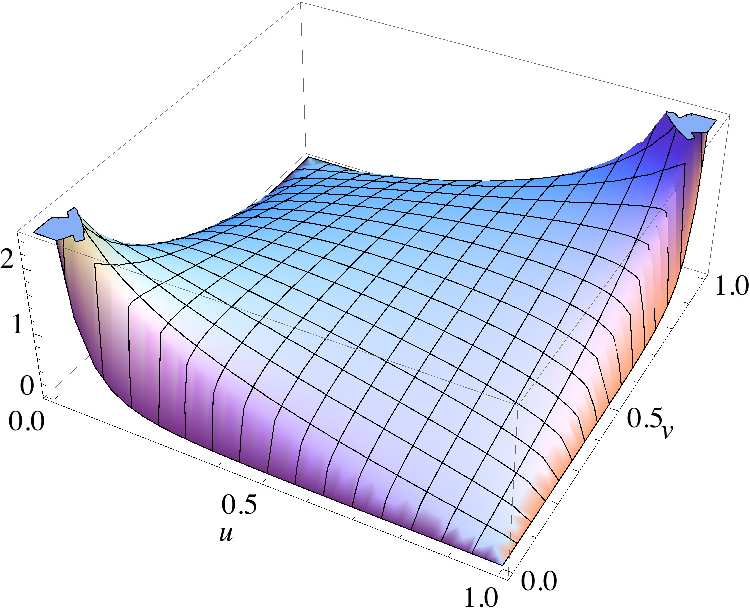
\includegraphics[scale=.35]{_pics/copulas/normal1.pdf}  
  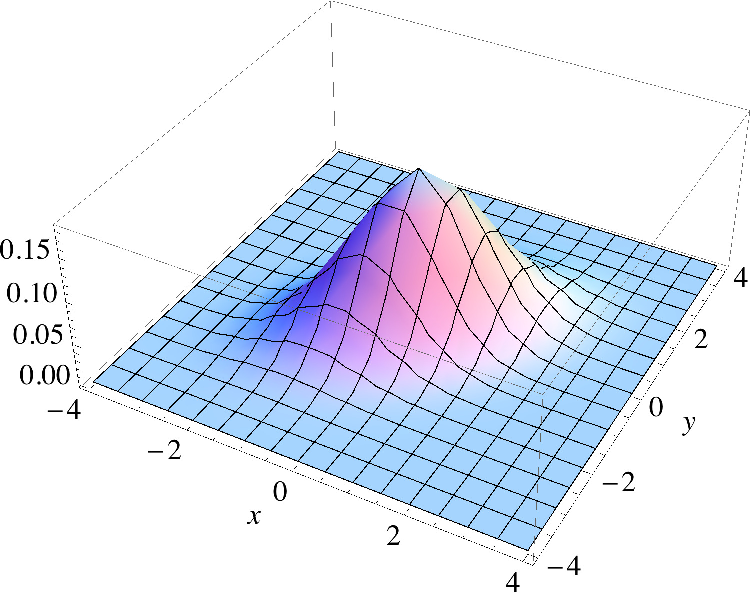
\includegraphics[scale=.35]{_pics/copulas/normal2.pdf}  
  \caption{Left: Density of the Gaussian (Normal) copula. Right:
    Density of the bivariate Normal distribution ($\rho=0.5$ in both
    cases).} 
  \label{fig:normalcopula}
\end{figure}

The Gaussian or Normal copula is
\begin{align}
    C^{Ga}_\Sigma(x) &= \frac{1}{(2\pi)^{d/2} |\Sigma|^{1/2}}
    \int_{-\infty}^{\Phi^{-1}(x_1)} \dots \int_{-\infty}^{\Phi^{-1}(x_d)}
    \exp \left\{
    -\frac{1}{2}y^\top \Sigma^{-1}y
    \right\}
    dy_1 \dots dy_d, \quad x\in \R^d.
    \end{align}

The copula density is
\begin{align}
    c^{Ga}_\Sigma(x) &= \frac{1}{(2\pi)^{d/2} |\Sigma|^{1/2}}
    \exp \left\{
    -\frac{1}{2}\begin{pmatrix} \Phi^{-1}(x_1) \\ \vdots \\ \Phi^{-1}(x_d) \end{pmatrix}^\top \Sigma^{-1} \begin{pmatrix} \Phi^{-1}(x_1) \\ \vdots \\ \Phi^{-1}(x_d) \end{pmatrix}
    \right\}
    \end{align}

Simplified notation bivariate Gaussian copula
\begin{align}
       C^{Ga}_\rho \{w, g(w)\} &= \Phi_\rho [\Phi^{-1}(w), \Phi^{-1}\{g(w)\}],
\end{align}
where $g(w): [0,1] \mapsto \mathbb{R}$ is defined above,
$\rho$ is the dependency parameter of a bivariate Gaussian copula,
$\Phi_\rho$ is bivariate normal distribution with mean 0 and covariance $\begin{bmatrix}1 & \rho \\ \rho & 1 \end{bmatrix}$,
$\Phi(\cdot)$ is CDF of standard normal,
$\phi(\cdot)$ is PDF of standard normal,
$\Phi^{-1}(\cdot)$ is quantile function of standard normal.

\natp{\em [I suggest to move the part below to the section where the
  formula for $R^h$ is discussed. Also, there is a simpler version
  that requires only univariate function evluations.]}

The bivariate $D_1 C^{Ga}\{w, g(w)\}$ is
\begin{align}
    D_1 C^{Ga}_\rho\{w, g(w)\} = \int_{-\infty}^{\Phi^{-1}\{g(w)\}} \phi_\rho\{
    \Phi^{-1}(w), u \}du \cdot \frac{1}{\phi\{\Phi^{-1}(w)\}}
    \end{align}
\begin{proof}
    \begin{align}
    D_1 C_\rho\{w, g(w)\}
    &= \left. \frac{\partial C_\rho\{w, g(w')\}}{\partial w}\right|_{w'=w}\\
    &= \left. \frac{\partial \Phi_\rho [\Phi^{-1}(w), \Phi^{-1}\{g(w)\}]}{\partial \Phi^{-1}(w)} \frac{\partial \Phi^{-1}(w)}{\partial w}\right|_{w'=w}\\
    &= \frac{1}{2\pi\rho} \int_{-\infty}^{\Phi^{-1}\{g(w)\}} \exp\left\{
        -\frac{1}{2(1-\rho^2)} \Phi^{-1}(w)^2 - 2\rho\Phi^{-1}(w)u + u^2
        \right\}du
        \cdot \frac{1}{\phi\{\Phi^{-1}(w)\}}
        \end{align}
    \end{proof}

% The bivariate Gaussian Copula density~$c^{Ga}\{w, g(w)\}$ is
% \begin{align}
%     c_\rho^{Ga}\{w, g(w)\} &= \frac{\partial D_1C_\rho^{Ga}\{w, g(w)\}}{\partial g(w)}\\
%                            &= \frac{\phi_\rho [\Phi^{-1}(w), \Phi^{-1}\{g(w)\}]}
%                             {\phi\{\Phi^{-1}(w)\}\phi[\Phi^{-1}\{g(w)\}]}
%     \end{align}


    
\subsubsection*{Hedge distribution}
\label{sec:hedge-distribution-gaussian}

Let $R^S\sim \Ncdf(\mu_S, \sigma_S^2)$ and $R^F\sim \Ncdf(\mu_F,
\sigma_F^2)$ and assume further that they are jointly normally
distributed with correlation $\rho$. Then,
\begin{equation*}
  R^h = R^S - h R^F \sim \Ncdf(\mu_S - h \mu_F, \sigma_s^2 + h^2
  \sigma_F^2 - 2\rho h \sigma_S \sigma_F).
\end{equation*}
More generally, if $R^k\sim F^k$, $k\in \{S,F\}$, then the
distribution of $R^h$ can be expressed with univariate
expressions: 
\begin{align*}
  \p(R^S-h R^F\leq x)
  &= 1-\E\left[ \p\left(R^F\leq \frac{R^S-x}{h}\big| R^S\right)\right] \\ %
  &= 1-\E\left[\p \left(\Ncdf^{(-1)}(F_F(R^F)) \leq
    \Ncdf^{(-1)}\left(F_F\left(\frac{R^S-x}{h}\right)\right) \Big|
    R^S\right)\right] \\%
  &= 1-\E\left[ \p\left(\rho \Ncdf^{(-1)}(F_S(R^S)) + \sqrt{1-\rho^2}
    \varepsilon \leq \Ncdf^{(-1)}\left(F_F\left(\frac{R^S-x}{h}\right)\right) \Big|
    R^S\right)\right]\\ %
  &= 1-\E\left[ \Ncdf \left(
    \frac{\Ncdf^{(-1)}\left(F_F\left(\frac{R^S-x}{h}\right)\right) -\rho
    \Ncdf^{(-1)}(F_S(R^S))} { \sqrt{1-\rho^2}}\right)\right]\\
  &= 1-\int_0^1  \Ncdf \left(
    \frac{\Ncdf^{(-1)}\left(F_F\left(\frac{F_S^{(-1)}(u)-x}{h}\right)\right) -\rho
    \Ncdf^{(-1)}(u)} { \sqrt{1-\rho^2}}\right) \,\dd u.
\end{align*}



\subsection{Archimedean copulas}
\label{sec:archimedean-copulas}

\begin{itemize}
\item A well-studied one-parameter family of copulas are the {\bf 
    Archimedean copulas}. 
\item Let $\phi:[0,1]\rightarrow[0,\infty]$ be a
  continuous and strictly decreasing function with $\phi(1)=0$ and
  $\phi(0)\leq\infty$.
\item  We define the {\bf pseudo-inverse} of $\phi$ as 
  \begin{equation*}
    \phi^{(-1)}(t)=
    \begin{cases}
      \phi^{-1}(t), &0\leq t\leq \phi(0),\\
      0, &\phi(0)<t\leq\infty.
    \end{cases}
  \end{equation*}
\item If, in addition, $\phi$ is convex, then the following function
  is a copula: 
  \begin{equation*}
    C(u,v)=\phi^{(-1)}(\phi(u)+\phi(v)).
  \end{equation*}
  \vspace*{-\baselineskip}
\item Such copulas are called {\bf Archimedean copulas}, and the
  function $\phi$ is called an {\bf Archimedean copula generator}. 
\item Examples of Archimedean copulas are the {\bf Gumbel} and the
  {\bf Clayton} copulas:
  \begin{align*}
    C_{\theta,{\rm Gu}}(u,v) &= \exp\left\{-((-\ln u)^\theta + (-\ln
                               v)^\theta)^{1/\theta}\right\},& 1\leq \theta<\infty,\\
    C_{\theta,{\rm Cl}}(u,v)&= (u^{-\theta} + v^{-\theta}
                              -1)^{-1/\theta}, & 0<\theta<\infty. 
  \end{align*}
\item In the case of the Gumbel copula, the independence copula is 
  attained when $\theta=1$ and the comonotonicity copula is attained
  as $\theta\rightarrow\infty$. 
\item Thus, the Gumbel copula interpolates between independence and
  perfect dependence.  
\item In the case of the Clayton copula, the independence copula is
  attained as $\theta\rightarrow 0$, whereas the comonotonicity
  copula is attained as $\theta\rightarrow\infty$. 
\end{itemize}

\subsection{Elliptical Copulas and normal variance mixtures}
\label{subsec:elliptical-copulae}


\providecommand{\bZ}{\ensuremath{\bm{Z}}}
\providecommand{\bU}{\ensuremath{\bm{U}}}
\providecommand{\bu}{\ensuremath{\bm{u}}}

See e.g.\ Theorem 3.22, Definition 3.26 and Theorem 3.28 of
\citep{McNeil2005}:
\begin{definition}
  A random vector $\bZ=(Z_0,\ldots, Z_d)^T$ follows an elliptical
  distribution if it has a representation
  \begin{equation*}
    \bZ\stackrel{\mathcal L}= G A \bU,
  \end{equation*}
  where $G>0$ is a scalar random variable, the so-called {\em mixing
  variable}, $A$ is a deterministic $(d+1)\times (d+1)$ matrix with
$A A^T:=\Sigma$, which in turn is a $(d+1)\times (d+1)$ nonnegative
definite symmetric matrix of rank $d+1$, and $\bU$ is a
$(d+1)$-dimensional random vector uniformly distributed on the unit
sphere $\mathcal S_{d+1}:=\{\bm{z}\in \R^{d+1}: \bm z^T \bm z=1\}$,
and $\bU$ is independent of $G$.
\end{definition}

A subclass of elliptical distributions are the so-called {\em normal
  variance mixtures (NVM)}, see Section 3.3 of \citep{McNeil2005}. For the
connection between NVM and elliptical distributions, see also Theorem
3.25 of \citep{McNeil2005}. 

\begin{definition}[Normal variance mixture (NVM)]
  The random vector $\mathbf X=(X_1, \ldots, X_k)^T$ follows a
  multivariate {\em normal variance mixture (NVM) distribution} if
  \begin{equation*}
    \mathbf X \stackrel{\mathcal L}{=} \mathbf \mu + \sqrt{W} A\mathbf
    Z, 
  \end{equation*}
  where
  \begin{enumerate}[(i)]
  \item $\mathbf Z\sim \Ncdf_k(\mathbf 0, I_k)$, i.e., $\mathbf Z$ are
    independent, standard normally distributed,
  \item $W\geq 0$ is a random variable independent of $\mathbf Z$,
  \item $A\in \R^{d\times k}$ and $\mathbf \mu\in R^d$ are a matrix
    and vector of constants, respectively. 
  \end{enumerate}
\end{definition}

It is easily observed that $\mathbf X|W=w \sim \Ncdf_d(\mathbf \mu,
w\Sigma)$, where $\sigma = A A'$.

In general, we will assume that $\Sigma$ is positive definite and that
$W>0$ $\pas$. Then, the density of $\mathbf X$ is given by
\begin{align*}
  f(\mathbf x) &= \int f_{\mathbf X|W} (\mathbf x|w)\, \dd H(w)\\
  &= \int \frac{w^{-d/2}} {(2\pi)^{d/2} |\Sigma|^{1/2}} \exp\left( -
    \frac{(\mathbf x-\mathbf \mu)' \Sigma^{-1} (\mathbf x-\mathbf
    \mu)} {2w} \right)\, \dd H(w),
\end{align*}
where $H$ is the distribution function of $W$.

Special cases:
\begin{itemize}
\item Normal distribution: $W$ constant
\item Student $t$ distribution: $W\sim \displaystyle Ig(1/2 \nu, 1/2
  \nu)$, where $Ig$ is an inverse gamma distribution
\item Symmetric generalised hyperbolic distribution: $W\sim
  N^{-}(\lambda, \chi, \psi)$ where $N^{-}$ refers to
  the generalised inverse Gaussian (GIG) distribution;
\item Normal inverse Gaussian (NIG): $W$ follows a GIG distribution
  with $\lambda=-0.5$.  
\end{itemize}

Copulas are obtained from elliptical distributions via Sklar's theorem
by transforming the margins to uniforms. 

\subsubsection*{Hedge distribution}
\label{sec:hedge-distribution-1}

Let $(R^S, R^F)$ follow a normal variance mixture, i.e., there exists a
decomposition such that
\begin{align*}
  R^S &=\mu_S + \sqrt{W} \sigma_S Z_1\\
  R^F &= \mu_F + \sqrt{W} \sigma_F (\rho Z_1 + \sqrt{1-\rho^2} Z_2),
\end{align*}
where $W$ is the mixing variable and $Z_1, Z_2$ are independent
standard normal variables. Then, $R^h$ follows a NVM distribution with
\begin{equation*}
  R^h = R^S - h R^F =  \mu_S - h \mu_F + \sqrt{W}
  \left((\sigma_S-h\sigma_F\rho)Z_1 -h \sqrt{1-\rho^2} 
    \sigma_F Z_2\right) = \mu_S - h \mu_F + \sqrt{W} Z_3,
\end{equation*}
where $Z_3\sim \Ncdf(0, \sigma_S^2 + h^2\sigma_F^2 - 2\rho
h\sigma_S \sigma_F)$. 

More generally, let $R^k\sim F^k$, $k\in \{S,F\}$ and write $V$
as the marginal distribution functions of the NVM distribution
components. Let $V^{(-1)}(F_S(R^S)) \stackrel{\mathcal L}{=} \sqrt{W}
Z_1$ and $V^{(-1)}(F_F(R^F)) \stackrel{\mathcal L}{=} 
\sqrt{W} \rho Z_1 + \sqrt{W} \sqrt{1-\rho^2} Z_2$, were $Z_1, Z_2$ are
independent standard normals. Then 
\begin{align*}
  \p(R^S-h R^F\leq x)
  &= 1-\E\left[ \p\left(R^F\leq \frac{R^S-x}{h}\big| R^S\right)\right] \\ %
  &= 1-\E\left[\p \left(V^{(-1)}(F_F(R^F)) \leq
    V^{(-1)}\left(F_F\left(\frac{R^S-x}{h}\right)\right) \Big|
    W, Z_1\right)\right] \\%
  &= 1-\E\left[ \p\left(\sqrt{W} \rho Z_1 + \sqrt{W} \sqrt{1-\rho^2}
    Z_2\leq V^{(-1)}\left(F_F\left(\frac{F_S^{(-1)}(V(\sqrt{W}
    Z_1))-x}{h}\right)\right) \Big| W, Z_1\right)\right]\\ %
  &= 1-\E\left[ \Ncdf \left(
    \frac{V^{(-1)}\left(F_F\left(\frac{F_S^{(-1)}(V(\sqrt{W}
    Z_1))-x}{h}\right)\right) -\rho \sqrt{W} Z_1} {
    \sqrt{W}\sqrt{1-\rho^2}}\right)\right]\\ 
  &= 1-\int_0^\infty \int_{-\infty}^{\infty} \Ncdf \left(
    \frac{V^{(-1)}\left(F_F\left(\frac{F_S^{(-1)}(V(\sqrt{w}
    z_1))-x}{h}\right)\right) -\rho\sqrt{w} z_1} { \sqrt{w}
    \sqrt{1-\rho^2}}\right) \, \varphi(z_1)\, f_W(w)\, \dd z_1\, \dd
    w.% \\
  % &= 1-\int_0^1 \int_{-\infty}^\infty  \Ncdf \left(
  %   \frac{V^{(-1)}\left(F_F\left(\frac{F_S^{(-1)}(u)-x}{h}\right)\right)
  %   -\rho V^{(-1)}(u)} { V^{(-1)}(u)/z_1
  %   \sqrt{1-\rho^2}}\right) \, \varphi(z_1)\, \dd z_1\, \dd
  %   u\\
\end{align*}
As in the Gaussian copula case, this expression contains evaluations
of only univariate distribution function. 

\subsection{Normal mean-variance mixtures}
\label{sec:normal-mean-variance}

Elliptical distributions are constrained to be symmetric. Extending
NVM's to normal mean-variance mixtures (NMVM) introduces skewness,
which may be more realistic for financial returns. We refer to Section
3.2.2 of \citep{McNeil2005} for more details.

\begin{definition}
The random vector $\mathbf {X}$ is said to have a (multivariate)
normal mean-variance mixture distribution if
\begin{equation*}
  \mathbf X \stackrel{\mathcal L}{=} \mathbf m(W) + \sqrt{W} A \mathbf Z,
\end{equation*}
where
\begin{enumerate}[(i)]
\item $\mathbf Z \sim \Ncdf_k (\mathbf 0, I_k)$;
\item $W\geq 0$ is a non-negative, scalar-valued random variable
  independent of $\mathbf Z$;
\item $A\in \R^{d\times k}$ is a matrix;
\item $\mathbf m:[0,\infty)\rightarrow \R^d$ is a measurable
  function. 
\end{enumerate}
We have
\begin{equation*}
  \mathbf X|W=w \sim \Ncdf_d(\mathbf m(w), w\Sigma),
\end{equation*}
where $\Sigma=A A'$. A possible concrete specification of $\mathbf
m(W)$ is
\begin{equation}
  \label{eq:9}
  \mathbf m(W) = \mathbf \mu + W\mathbf \gamma,
\end{equation}
where $\mathbf\mu$ and $\mathbf\gamma$ are vectors in $\R^d$. If
$\mathbf\gamma=0$, then the distribution is a NVM. 

A special case are the {\em generalized hyperbolic (GH)
  distributions}, which a NMVM's with mean specification (\ref{eq:9})
and mixing distribution $W\sim N^{-}(\lambda, \chi, \psi)$, a
generalised inverse Gaussian (GIG) distribution. We write $\mathbf
X\sim \text{GH}_d(\lambda, \chi, \psi, \mathbf \mu, \Sigma,
\mathbf\gamma)$. The specification is not unique in the sense that
scaled versions of the parameters described the same
distribution. 

A different parameterization is obtained using the parameters $\alpha,
\delta, \Delta, \mathbf \beta$:
\begin{equation*}
  \Delta = |\Sigma|^{-1/3} \Sigma, \quad \mathbf\beta = \Sigma^{-1}
  \mathbf \gamma, \quad \delta =\sqrt{\chi |\Sigma|^{1/d}}, \quad
  \alpha = \sqrt{|\Sigma|^{-1/d} (\psi + \mathbf\gamma' \Sigma^{-1}
    \mathbf\gamma)}. 
\end{equation*}
It is not uncommon to restrict $|\Delta|=1$. The parameters have the
following interpretation: $\mu$ is the location parameter, $\delta$
the scale parameter, $\beta$ the skewness parameter and $\alpha$ and
$\lambda$ are shape parameters. 

If $\alpha, \delta, \Delta, \mathbf\beta$ is used, then
\begin{equation*}
  \Sigma = \Delta, \quad \mathbf\gamma = \Delta\mathbf \beta, \quad
  \chi = \delta^2, \quad \psi = (\alpha^2 - \mathbf\beta' \Delta
  \mathbf\beta). 
\end{equation*}
Amongst several special cases, we consider the NIG and the skewed $t$
distributions:
\begin{itemize}
\item $\lambda=-1/2$ gives rise to the NIG distribution
\item $\lambda=-1/2 \nu$, $\chi=\nu$, $\psi=0$ gives rise to an
  asymmetric or skewed $t$ distribution. The multivariate $t$
  distribution is obtained as $\mathbf \gamma\rightarrow 0$. 
\end{itemize}


A different parameterization is obtained by setting
\begin{equation*}
  \mathbf \beta = \Sigma^{-1}\mathbf \gamma, \quad \delta=\sqrt\chi,
  \quad \alpha = \sqrt{\psi + \mathbf \gamma' \Sigma^{-1} \mathbf
    \gamma}, 
\end{equation*}
satisfying the constraints $\delta\geq0$, $\alpha^2 > \mathbf \beta'
\Sigma\mathbf\beta$ if $\lambda>0$; $\delta>0$, $\alpha^2>
\mathbf\beta' \Sigma\mathbf \beta$ if $\lambda=0$; and $\delta>0$,
$\alpha^2\geq \mathbf\beta' \Sigma \mathbf \beta$ if $\lambda<0$. 



\end{definition}


\subsection{Normal inverse Gaussian factor copula model}
\label{sec:norm-inverse-gauss-1}

Literature on NIG, factor copulas and fitting of copulas:
\begin{itemize}
\item \citep{Kalemanova2007}: NIG factor model, calibrated to CDO's
\item \citep{Genest1987,Genest1993}: ``Method of moments'' for
  nonparametric estimation of copula parameters; mainly refers to
  Kendall's tau or Spearman's rho
\item \citep{Patton2012,Oh2013}: Factor copula models (in particular
  skewed $t$), estimated with ``method of moments'' involving
  Spearman's rank correlation, and $0.05, 0.1, 0.9, 0.95$ quantile
  dependence measures
\end{itemize}


\subsubsection{Normal inverse Gaussian distribution}
\label{sec:norm-inverse-gauss-2}

It was established in the previous section that a multivariate normal
inverse Gaussian (NIG)
distribution is a normal variance mixture. Here the random components 
have a joint scalar mixing variable. 
An additional copula model can be derived as a factor model from the
NIG distribution: under certain conditions, its distribution type is
preserved under linear combinations. This property, together with 
its infinite divisibility, allow for the construction of L\'evy
processes from NIG distributions.

\begin{figure}[t]
  \centering
  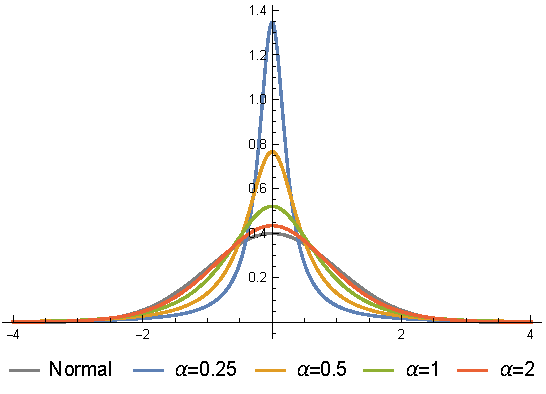
\includegraphics[scale=.85]{_pics/nigpdf1.pdf}
  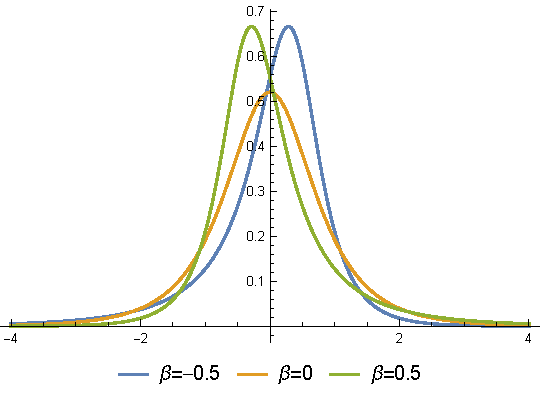
\includegraphics[scale=.85]{_pics/nigpdf2.pdf}
  \caption{Standardised NIG's density functions, i.e., $\mu$ and
    $\delta$ yield zero expectation and unit variance. Left:
    $\beta=0$; right: $\alpha=1$. With increasing $\alpha$, the
    standardised NIG converges to a normal distribution.} 
  \label{fig:nigpdf}
\end{figure}
% This last point is easily seen by observing that the mixing variable
% has a mean of 1 and its variance converges to zero.

Following \citep{BarndorffNielsen1997}, a normal inverse Gaussian
(NIG) distribution has density function
\begin{equation*}
  g(x; \alpha,\beta, \mu, \delta) = \frac{\alpha}{\pi} \e^{\delta
    \sqrt{\alpha^2-\beta^2} -\beta\mu} \frac{1}{q((x-\mu)/\delta)}
  K_1\left[\delta \alpha q\left(\frac{x-\mu}{\delta}\right) \right]
  \e^{\beta x},\quad x>0,
\end{equation*}
where $q(x) = \sqrt{1+x^2}$ and where $K_1$ is the modified Bessel
function of third order and index $1$. The parameters satisfy $0\leq
|\beta|\leq \alpha$, $\mu\in \R$ and $\delta>0$. The parameters have
the following interpretation: $\mu$ and $\delta$ are location and
scale parameters, respectively, $\alpha$ determines the heaviness of
the tails and $\beta$ determines the degree of asymmetry. If
$\beta=0$, then the distribution is symmetric around $\mu$. Figure
\ref{fig:nigpdf} shows examples of NIG densities. 

The moment-generating function of the NIG distribution is given by
\begin{equation*}
  M(u; \alpha, \beta, \mu, \delta) = \exp\left( \delta
    \left(\sqrt{\alpha^2-\beta^2} - \sqrt{\alpha^2 - (\beta +
        u)^2}\right) + \mu u\right). 
\end{equation*}
As a direct consequence, moments are easily calculated with the
expectation and variance of the NIG distribution being
\begin{align}
  \label{eq:4}
  \mathbb E X &= \mu + 
                \frac{\delta \beta}{\sqrt{\alpha^2-\beta^2}}\\
  \label{eq:5}
  \text{Var}(X) &= \frac{\alpha^2\delta}{(\alpha^2-\beta^2)^{3/2}}.
\end{align}


Let $\text{IG}(\delta,\gamma)$ denote the {\em inverse Gaussian
  distribution} with density function\footnote{%
  The density of the IG distribution in {\tt Mathematica} is given as
  \begin{equation*}
    f(x) = \sqrt{\frac{\lambda}{x^3}} \frac{1}{\sqrt{2\pi}}
    \e^{-\frac{\lambda(x-\mu)^2}{2 x\mu^2}},\quad x>0,
  \end{equation*}
  with parameters $\mu=\delta/\gamma$ and $\lambda=\delta^2$. 
  }%
\begin{equation}
  \label{eq:2}
  d(w; \delta, \gamma) = \frac{1}{\sqrt{2\pi}} \exp(\delta \gamma)
  w^{-3/2} \exp(-\frac{\delta^2/w + \gamma^2 z}{2}). 
\end{equation}
The $\text{NIG}(\alpha, \beta, \mu\, \delta)$ distribution is a normal
variance-mean mixture: $X$ follows an
$\text{NIG}(\alpha,\beta,\mu,\delta)$ distribution if $X$ conditional
on $W$ follows a normal distribution with mean $\mu+\beta W$ and
variance $W$, i.e., 
\begin{equation*}
  X|W\stackrel{\mathcal L}\sim \Ncdf(\mu + \beta W, W),
\end{equation*}
where $W$ follows an $\text{IG}(\delta, \sqrt{\alpha^2-\beta^2})$
distribution. 

It is easily seen from the moment-generating function that linear
combinations of NIG random variables are again NIG-distributed
provided they share the parameters $\alpha$ and $\beta$. Let $X_i\sim
\text{NIG}(\alpha, \beta, \mu_i, \delta_i)$, $i=1,2$, be
independent NIG variables. Then, 
\begin{equation*}
  \E\left[\e^{u(X_1+X_2)}\right] = \E\left[\e^{u X_1}\right]
  \E\left[\e^{u X_2}\right] = \exp\left((\delta_1+\delta_2)
    \left(\sqrt{\alpha^2-\beta^2} - \sqrt{\alpha^2 -
        (\beta+u)^2}\right) + (\mu_1+\mu_2) u\right),
\end{equation*}
hence $X_1+X_2\sim \text{NIG}(\alpha, \beta, \mu_1+\mu_2,
\delta_1+\delta_2)$. (This is also a direct consequence from the
properties of 
the normal inverse Gaussian L\'evy process $X_t$, which may be
represented as Brownian motion with a random time change,
\begin{equation*}
  X_t = B_{W_t} + \mu t,
\end{equation*}
where $B=(B_t)_{t\geq 0}$ is a Brownian motion and $W=(W_t)_{t\geq 0}$
is a L\'evy process with density given by \eqref{eq:2}. The random
variable $W_t$ can be interpreted as a first-passage time of an
independent Brownian motion $\overline B$, i.e., $W_t=\inf\{s>0:
\overline B_s + \sqrt{\alpha^2-\beta^2}s = \delta t\}$.)

As a consequence, the NIG distribution gives rise to two copulas:
\begin{itemize}
\item a copula determined from a linear combination of independent NIG
  random variables with identical parameters $\alpha, \beta$
  (essentially a factor model);
\item a copula determined from the multivariate normal-mean-variance
  mixture, which is a linear combination of normal random variables
  scaled by one scalar inverse Gaussian random variable.
\end{itemize}

\subsubsection{NIG factor copula}
\label{sec:nig-factor-copula}

We consider a simple factor model consisting of NIG-distributed random
variables.
\begin{proposition}
  \label{prop:NIG}
  Let $Z\sim \text{NIG}(\alpha, \beta, \mu, \delta)$ and
  $Z_i\sim \text{NIG}(\alpha, \beta, \mu_i, \delta_i)$,
  $i=1,\ldots, n$ be independent NIG-distributed random
  variables. Then (i) 
  $X_i = Z + Z_i\sim \text{NIG}(\alpha,\beta,\mu+\mu_i,
  \delta+\delta_i)$ and (ii)
  \begin{align}
    \text{Cov}(X_i,X_j) &= \text{Var(Z)},\nonumber\\
    \text{Corr}(X_i,X_j) &= \frac{\delta}{\sqrt{(\delta+\delta_i)
                           (\delta+\delta_j)}}. \label{eq:6}
  \end{align}
\end{proposition}
\begin{proof}
  \begin{enumerate}[(i)]
  \item This follows directly from the moment-generating function. 
  \item For the covariance,
    \begin{align*}
      \text{Cov}(X_i,X_j)
      &= \E[(Z+Z_i) (Z+Z_j)] - \E[Z+Z_i] \E[Z+Z_j]\\
      &= \E[Z^2] -(\E Z)^2.
    \end{align*}
    The correlation is determined directly from \eqref{eq:5}. 
  \end{enumerate}
\end{proof}

The NIG factor copula is obtained by transforming the margins to
uniforms (see Sklar's Theorem).

The NIG factor copula function can be written as \citep{krupskii2013factor}:
\begin{align}
  C_{R^S, R^F}\{F_{R^S}(r^S), F_{R^F}(r^F)\} = \int_\mathbb{R}
  F_{Z_1}\{F_{X_1}^{-1} \circ F_{R^S}(r^S) -z\} \cdot
  F_{Z_2}\{F_{X_2}^{-1} \circ F_{R^F}(r^F) -z\} \cdot
  f_Z(z) dz
  \end{align}

The Spearman rho of NIG factor copula is
\begin{align}
  \rho_S = 12 \int \int \int_{\mathbb{R}^3}
  F_{X_1}(x_1) \cdot
  F_{X_2}(x_2) \cdot
  f_{Z_1}(x_1-z) \cdot
  f_{Z_2}(x_2-z) \cdot
  f_Z(z) dx_1 dx_2 dz - \frac{1}{48}
  \end{align}

\begin{proof}
  \begin{align}
  \rho_S(R^S, R^F) &= \rho\{F_{R^S}(R^S), F_{R^F}(R^F)\} \\
    &= \rho\{F_{X_1}(X_1), F_{X_2}(X_2)\} \\
    &= 12 \cdot \mathbb{E}\{F_{X_1}(X_1) \cdot F_{X_2}(X_2) \} - \frac{1}{48}\\
    &= 12 \cdot \int \int_{\mathbb{R}^2} F_{X_1}(X_1) \cdot F_{X_2}(X_2) dF_{X_1,X_2}(x_1,x_2)\\
    \end{align}
  Because
  \begin{align}
    F_{X_1,X_2}(x_1,x_2) &= \mathbb{P}(X_1 \leq x_1, X_2 \leq x_2)\\
    &= \mathbb{P}(Z_1 \leq x_1 - Z, Z_2 \leq x_2 - Z) \\
    &= \int_\mathbb{R}\mathbb{P}(Z_1 \leq x_1 - z) \cdot \mathbb{P}(Z_2 \leq x_2 - z) \cdot f_Z(z) dz,
    \end{align}
  so,
  \begin{align}
    \rho_S(R^S, R^F) = 12 \cdot \int \int \int_{\mathbb{R}^3} F_{X_1}(x_1) \cdot F_{X_2}(x_2) \cdot f_{Z_1}(x_1 -z) \cdot f_{Z_2}(x_2 -z) \cdot f_{Z}(z) dx_1 dx_2 dz -\frac{1}{48}
    \end{align}
  \end{proof}

\subsubsection{Fitting the NIG factor model}
\label{sec:fitt-nig-distr}

In this section we assume that the marginal distributions are NIG. 

Given that the parameters $\alpha, \beta, \mu, \delta$ denote tail
heaviness, skewness, location and scale, one can fit the NIG
distribution by matching the first four moments. Let
$\hat\mu_r=\frac{1}{n} \sum_{i=1}^n x_i^r$ denote the $r$-th moment of
the sample $x_1, \ldots, x_n$. Then moment-matching the NIG
distribution corresponds to solving for $\alpha, \beta, \mu, \delta$
the system of equations
\begin{equation*}
  \begin{pmatrix}
    \frac{\partial}{\partial u} M(u; \alpha, \beta, \mu,
    \delta)|_{u=0}\\[5pt]
    \frac{\partial^2}{\partial u^2} M(u; \alpha, \beta, \mu,
    \delta)|_{u=0}\\[5pt]
    \frac{\partial^3}{\partial u^3} M(u; \alpha, \beta, \mu,
    \delta)|_{u=0}\\[5pt]
    \frac{\partial^4}{\partial u^4} M(u; \alpha, \beta, \mu,
    \delta)|_{u=0}\\
  \end{pmatrix}
  =
  \begin{pmatrix}
    \hat\mu_1\\[5pt]
    \hat\mu_2\\[5pt]
    \hat\mu_3\\[5pt]
    \hat\mu_4
  \end{pmatrix}
\end{equation*}


Bivariate data, as present in our case, can be
fit by moment-matching involving the parameters $(\alpha, \beta,
\mu_1, \mu_2, \delta_1, \delta_2)$ and then fitting $\delta$ of the
joint factor via the empirical correlation. Without loss of
generality, we set $\mu=0$. Then, $\alpha, \beta,
\mu_i,\tilde\delta_i$, $i=1,2$, are determined from 
\begin{align*}
  \min_{\alpha, \beta, \mu_1, \mu_2, \tilde\delta_1, \tilde\delta_2}
  \sqrt{\sum_{k=1}^2 \sum_{r=1}^4
  \left(\hat\mu_{r,k}-\frac{\partial^r}{\partial u^r} M(u; \alpha, \beta,
  \mu_k, \tilde\delta_k)\Big|_{u=0}\right)^2}.
\end{align*}
Here, $\tilde\delta_k$ refers to the scale parameter of
$X_k$. The scale parameters of the independent NIG components $Z_k$,
$k=1,2$, are obtained as $\delta_k=\delta-\tilde \delta_k$ after
solving $\delta$ from \eqref{eq:6}, which fixes the dependence between
the margins. Figure \ref{fig:nig} shows
histograms and the fitted NIG densities of the Bitcoin reference rate
(BRR) returns and the Bitcoin Futures contract returns (BTCF). 


\begin{figure}[t]
  \centering
  % 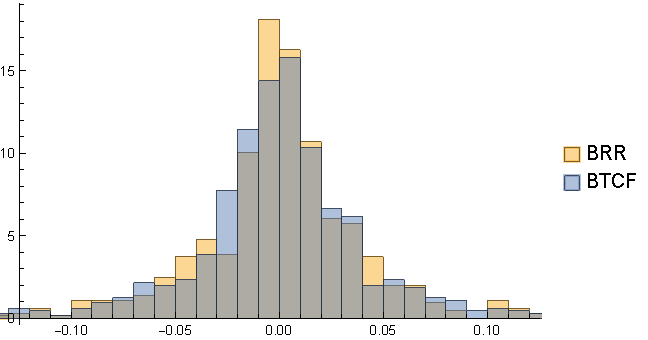
\includegraphics[scale=.7]{_pics/fittedNIG.pdf} 
  % 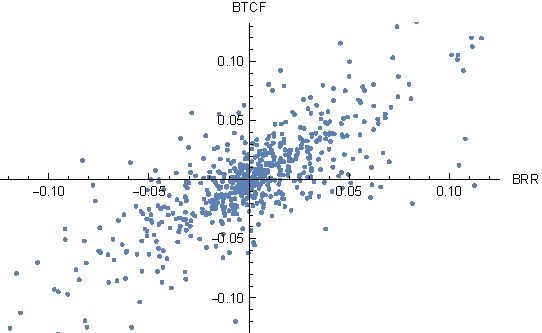
\includegraphics[scale=.7]{_pics/scatter.pdf}
  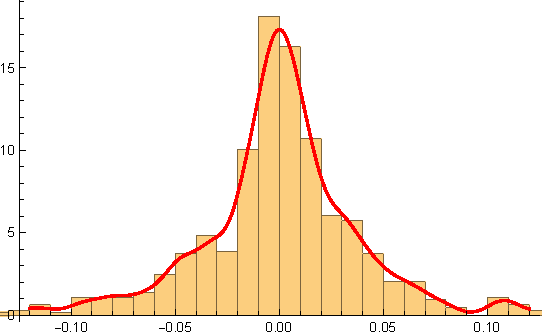
\includegraphics[scale=.55]{_pics/rbrr.pdf} \ \ 
  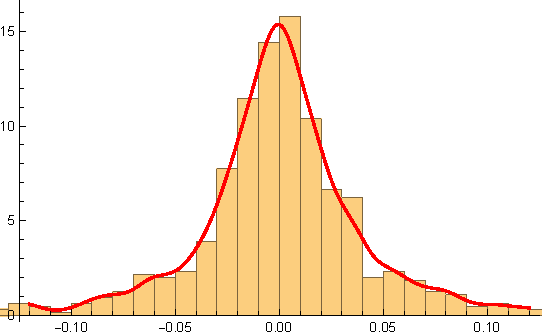
\includegraphics[scale=.55]{_pics/rbtc.pdf}\ \ 
  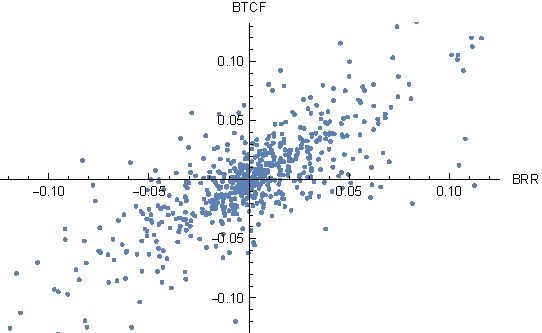
\includegraphics[scale=.4]{_pics/scatter.pdf}
  \caption{BRR and BTCF return distributions (empirical and fitted to
    NIG) as well as scatter plot.}
  \label{fig:nig}
\end{figure}

\subsubsection{Fitting the NIG factor copula}
\label{sec:fitting-nig-factor}

If the margins are not NIG-distributed, then the NIG factor copula
model is calibrated by the so-called ``method of moments'' as
described by \citep{Oh2013}. In this setting, Spearmans' rho (rank
correlation) and quantile dependence measures at the $0.05, 0.1, 0.9,
0.95$ quantiles are calibrated against the empirical
counterparts. Spearman's rho and quantile dependence of a pair $(X,Y)$
with copula $C$ are defined as 
\begin{align}
  \rho_S &= 12 \int\int_{I^2} C(u,v)\, \dd u\, \dd v-3\label{eq:10}\\
  \lambda_q &=
  \begin{cases}
    \p(F_X(X)\leq q| F_Y(Y)\leq q) = \displaystyle \frac{C(q,q)}{q},
    &\text{ if } q\in (0,0.5],\\
    \p(F_X(X)>q|F_Y(Y)>q) =\displaystyle \frac{1-2q+C(q,q)} {1-q},
    &\text{ if } q\in (0.5,1). 
  \end{cases}
\end{align}
The empirical counterparts are
\begin{align*}
  \hat\rho_S &= \frac{12}{n} \sum_{k=1}^n \hat F_X(x_k) \hat F_Y(y_k)
               -3,\\
  \hat\lambda_q &=
                  \begin{cases}
                    \displaystyle\frac{1}{n} \sum_{k=1}^n \frac{\1_{\{\hat
                        F_X(x_k)\leq q, \hat F_Y(y_k)\leq q\}}} {q},
                    &\text { if } q\in (0, 0.5],\\
                    \displaystyle \frac{1}{n} \sum_{k=1}^n
                    \frac{\1_{\{\hat F_X(x_k)>q, \hat F_Y(y_k)>q\}}}
                    {1-q}, &\text { if } q\in (0.5,1). 
                  \end{cases}
\end{align*}
Here, the empirical distribution function is defined such that the
data lie strictly in the interior of the unit cube (see \citep{Oh2013}
and \citep[p.\ 232]{McNeil2005}):
\begin{equation*}
  \hat F(x) = \frac{1}{n+1} \sum_{k=1}^n \1_{\{x_k\leq x\}}. 
\end{equation*}
Convergence of the sample measures to the population counterparts is
established by \citep{Fermanian2004}.

Denote the {\em standardised\/} NIG distribution function (i.e.,
expectation $0$ and variance $1$) by $F(\cdot; \alpha, \beta)$. In this case
$\delta(\alpha,\beta)=\displaystyle\frac{(\alpha^2-\beta^2)^{3/2}}{\alpha^2}$
and $\mu(\alpha,\beta)=\displaystyle - \frac{\delta \beta}
{\sqrt{\alpha^2-\beta^2}} = \frac{\beta^3}{\alpha^2} -\beta$. In the
factor model setting, the parameters $\alpha, \beta$ and $\delta$ are
calibrated, where $\delta$ refers to the scaling parameter of the
latent variable $Z$. 



Denote the margins by
$U_i\sim U(0,1)$, $i=1,2$. The factor model of Proposition
\ref{prop:NIG} is 
obtained by transforming the uniform margins to standardised NIG
distributions by setting  
$X_i:=F^{(-1)}(U_i; \alpha, \beta, \mu, \delta+\delta_i)$ with 
$\delta+\delta_i=\displaystyle \frac{(\alpha^2-\beta^2)^{3/2}}
{\alpha^2}$ and $\mu=\displaystyle -\frac{(\delta+\delta_i)\beta}
{\sqrt{\alpha^2-\beta^2}} = -\frac{(\alpha^2-\beta^2) \beta}
{\alpha^2}=\frac{\beta^3}{\alpha^2}-\beta$. Here, $\delta$ refers to
the scaling factor of the latent variable $Z$. In 
this case, $\E X_i=0$ and $\text{Var}(X_i)=1$.

Calibrating the NIG factor copula corresponds to minimising the
root mean square error of the sample and distribution copula measures: 
\begin{equation*}
  \min_{\alpha, \beta, \delta} \sqrt{ (\rho_S - \hat\rho_S)^2 +
    (\lambda_{0.05}-\hat\lambda_{0.05})^2 + 
    (\lambda_{0.1}-\hat\lambda_{0.1})^2 + 
    (\lambda_{0.9}-\hat\lambda_{0.9})^2 + 
    (\lambda_{0.95}-\hat\lambda_{0.95})^2}
\end{equation*}

To avoid numerical calculation of $\rho_S$ in Equation
\eqref{eq:10}, which requires integrating the copula
function, we approximate $\rho_S$ by the rank correlation for the
Gaussian copula (see \citep[p.\ 215]{McNeil2005}), 
\begin{equation}
  \label{eq:11}
  \rho_S(X_1,X_2) = \frac{6}{\pi} \arcsin \frac{1}{2}\rho. 
\end{equation}
This is justified if $\beta$ is close to zero and for sufficiently
large values of $\alpha$, as the NIG converges to the normal
distribution as $\alpha\rightarrow\infty$. It turns out that the
approximation is close even for $\alpha$ in the order of e.g.\ $4$.

\natp{\em \bf [Possibly compute AIC in order to compare the
  calibration performance across models?]}

\paragraph{Bitcoin data}

The copula parameters obtained in the calibration of the Bitcoin data
are $\alpha=3.1354$, $\beta=0.121548$, $\delta=2.53221$. The NIG rank
correlation obtained with these parameters is $\rho_S=0.8011$, whereas
the Gaussian approximation of \eqref{eq:11} gives $0.7958$.

\begin{table}[t]
  \centering
  \begin{tabular}{|c||c|c|}
    \hline %
    Measure & Empirical & Calibrated\\\hline
    $\rho_s$ & 0.7337 & 0.7958\\
    $\lambda_{0.05}$ & 0.5581 & 0.5290\\
    $\lambda_{0.1}$ & 0.6357 & 0.5871\\
    $\lambda_{0.9}$ & 0.6202 & 0.5896\\
    $\lambda_{0.95}$ & 0.5891 & 0.5325\\\hline
  \end{tabular}
  \caption{Empirical versus calibrated dependence measures. The
    calibrated parameters are $\alpha=3.1354$, $\beta=0.121548$,
    $\delta=2.53221$. }
  \label{tab:nigcopula}
\end{table}

\begin{figure}[t]
  \centering
  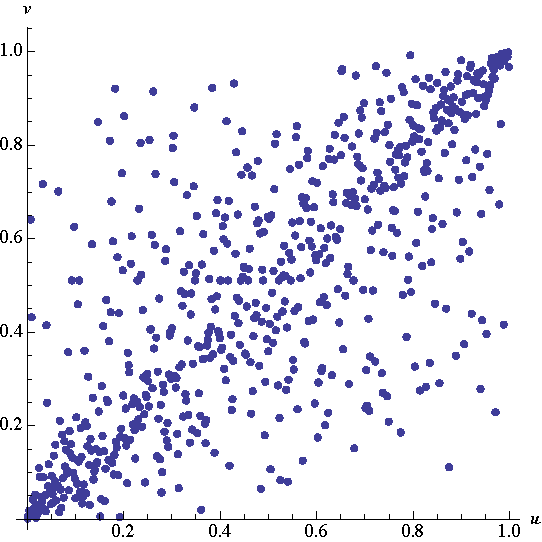
\includegraphics[scale=.5]{_pics/copula_nig1.pdf}\ \ \ \ \ 
  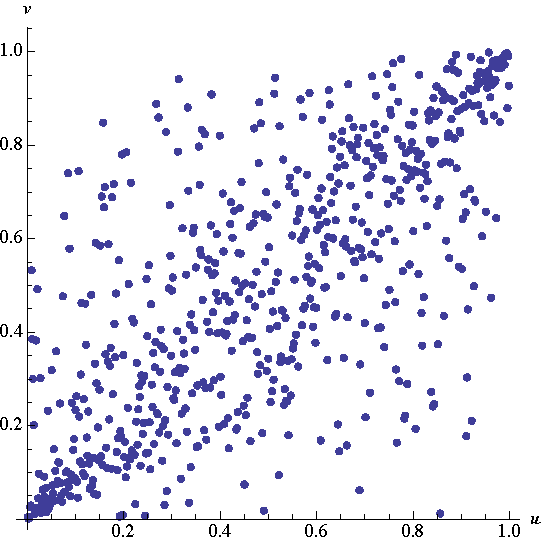
\includegraphics[scale=.5]{_pics/copula_nig2.pdf}
  \caption{Left: Scatter plot of empirical copula; right: scatter plot
    of simulated sample with calibrated parameters.}
  \label{fig:copula_nig}
\end{figure}



% Denote the $r$-th
% empirical uncentered moment of $i$-th NIG-transformed margin by
% \begin{equation}
%   \label{eq:8}
%   \hat\mu_{i,r}(\alpha, \beta, \mu,\delta) := \frac{1}{n}
%   \sum_{j=1}^n 
%   F^{(-1)}(u_{i,j}; \alpha,\beta,\mu, \delta)^r,
% \end{equation}



% Given the interpretation of the parameters -- $\alpha$ as the tail
% heaviness, $\beta$ as the degree of asymmetry, and $\delta$
% determining the correlation -- calibrating the bivariate factor model
% is the achieved by minimising the RMSE of the third and
% fourth moments and the correlation between the model and the data: 
% \begin{multline*}
%   \min _{\alpha, \beta, \delta, \delta_1, \delta_2}
%   \left(\text{Corr}(F^{(-1)}(U_1; \alpha, \beta, \mu,\delta+\delta_1),
%   F^{(-1)}(U_2; \alpha, \beta, \mu, \delta+\delta_2)-\frac{\delta}
%   {\sqrt{(\delta+\delta_1) (\delta+\delta_2)}}\right)^2\\
% + \sum_{i=1}^2 \sum_{r=3}^4 
%   \left(\hat\mu_{i,r}(\alpha,\beta,\delta+\delta_i) -
%     \frac{\partial^r}{\partial u^r} M(u; \alpha,  
%     \beta,\mu, \delta+\delta_i)\Big|_{u=0}\right)^2 \text{, subject
%     to } \delta+\delta_i=\displaystyle \frac{(\alpha^2-\beta^2)^{3/2}}
% {\alpha^2},
% \end{multline*}
% with $\mu=\displaystyle\frac{\beta^3}{\alpha^2}-\beta$. 

% This implies that $\delta_1=\delta_2$. A standardised multivariate
% model would therefore be homogeneous with one correlation coefficient
% for all pairwise margins. Different correlations would be achieved 
% by loosening the constraint of unit variances. Re-writing, with
% $\tilde\delta := \delta + \delta_1 = \displaystyle
% \frac{(\alpha^2-\beta^2)^{3/2}} {\alpha^2}$ gives 
% \begin{equation*}
%   \min _{\alpha, \beta, \delta}
%   \left(\text{Corr}(F^{(-1)}(U_1; \alpha, \beta, \mu,\tilde\delta),
%   F^{(-1)}(U_2; \alpha, \beta, \mu, \tilde\delta)-\frac{\delta}
%   {\tilde\delta}\right)^2 %
% + \sum_{i=1}^2 \sum_{r=3}^4 
%   \left(\hat\mu_{i,r}(\alpha,\beta,\tilde\delta) -
%     \frac{\partial^r}{\partial u^r} M(u; \alpha,  
%     \beta,\mu, \tilde\delta) \Big|_{u=0}\right)^2.
% \end{equation*}

\clearpage
\subsubsection{NIG quantiles}
\label{sec:nig-quantiles}

Calibration of the copula model requires an efficient implementation
of the NIG quantile function, see Equation (\ref{eq:8}). One way of
implementing this is via the so-called {\em Cornish-Fisher expansion}
(CF expansion), \citep{Cornish1938}. The quantile function of a
distribution function is approximated by the known quantile of another
distribution (e.g.\ normal or $t$-distribution) and expanded using the
cumulants of the 
desired distribution. The CF expansion is a popular choice for
calculating the value-at-risk of financial portfolios when no closed
formula of the quantile function exists, see e.g.\
\citep{Jaschke2002,Lau2015}.  The version of the CF expansion used
here follows \citep{Abramowitz1972}, 26.2.49-26.2.51.

The CF expansion may not converge in the sense as a Taylor
expansion does, so other techniques such as Monte Carlo simulation may
produce better results, especially in the tails. However, the CF
expansion is extremely fast, so that we use it for calibrating the
copula model and switch to Monte Carlo simulation for calculating the
optimal hedge ratio.

\begin{figure}[t]
  \centering
  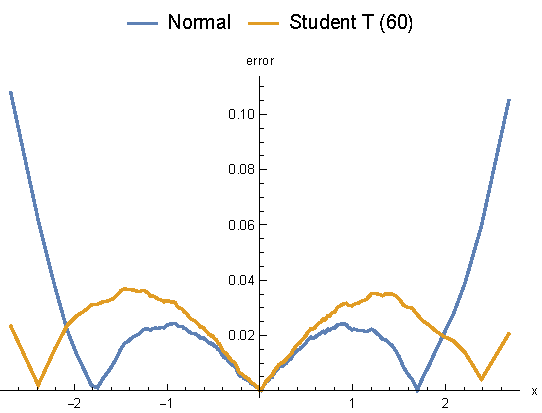
\includegraphics[scale=.5]{_pics/CFerror.pdf}
  \caption{blub}
  \label{fig:CF_NIG}
\end{figure}

Figure




\natp{Simulation produces better results but requires more
  computational power. Hence, use CF for calibration, which performs
  worse in the tails, and simulation in the hedge calculation / risk
  measure calculation. Use importance sampling.}


\subsubsection{Hedge calculation in the NIG factor model}
\label{sec:hedge-calc-nig}

Optimising for the hedge quantity $h$ requires fast calculations of
the hedge distribution function \eqref{eq:3}. The position obtained
from hedging Bitcoin with $h$ units of the Bitcoin future returns
\begin{equation*}
  R^h = X_1 - h X_2 = Z + Z_1 - h Z - h Z_2 = (1-h) Z + Z_1 - h Z_2,
\end{equation*}
with $Z, Z_1, Z_2$ independent NIG-distributed random
variables. Without loss of generally, set $\mu=0$. Because of the
scaling with $1-h$ and $h$, $R^h$ will not follow an NIG distribution,
unless $h=0$.  A direct calculation of the distribution function is
achieved by numerically computing the integral
\begin{equation*}
  \p(R^h\leq x) = \int_0^\infty \int_0^\infty \int_0^\infty
  \Ncdf(y; \mu_1 - h \mu_2 + \beta w_1 - h w_2, (1-h)^2 w + w_1 + h^2
  w_2)\, f_W(w)\, f_{W_1}(w_1)\, f_{W_2} (w_2)\, \dd w\, \dd w_1\, \dd w_2,
\end{equation*}
where $\Ncdf(x; \mu, \sigma^2)$ denotes the normal distribution
function with expectation $\mu$ and variance $\sigma^2$, and
$f_W, f_{W_1}, f_{W_2}$ are the inverse Gaussian density functions of the
scaling variables $W$, $W_1$ and $W_2$ with parameters
$\delta, \delta_1, \delta_2$ and $\sqrt{\alpha^2-\beta^2}$. 

However, for determining the optimal hedge parameter $h$, numerical
computation of the three-fold integral may be slow, compared to other
methods that make explicit use of the simple form of the
moment-generating function.  The following two methods achieve a much
faster computation for the NIG factor model.  The first method uses
Fourier inversion to calculate the density from the characteristic
function. The second method approximates the distribution of $R^h$ by
an NIG distribution.  Both methods use the moment-generating function
of $R^h$, which is given by
\begin{align}
  \varphi_h(u):=\E\left[\e^{u R^h}\right]
  &= \E\left[ \e^{u[(1-h) Z + Z_1 -h Z_2]}\right] %
    = \E\left[ \e^{u(1-h) Z}\right]\, \E\left[ \e^{u Z_1}\right] \,
    \E\left[ \e^{-u h Z_2}\right]\nonumber\\
  &=M\left(u;\frac{\alpha}{1-h}, \frac{\beta}{1-h}, (1-h)\mu,
    (1-h)\delta\right)\,
    M\left(u; \alpha, \beta, \mu_1, \delta_1\right)\,
    M\left(-u; \frac{\alpha}{h}, \frac{\beta}{h}, h\mu_2,
    h\delta_2\right).
    \label{eq:7}
\end{align}


\natp{Add copula stuff; here the assumption is still that $R_S$ and
  $R_F$ are NIG.}

\paragraph*{Calculation via Fourier inversion}
\label{sec:calc-via-four}

Because of the simple form of the moment-generating function
\eqref{eq:7}, the density $f$ of $R^h$ can be calculated numerically
using the inverse Fourier transform of the characteristic function
$\varphi(u) $:
\begin{equation*}
  f(x) = \frac{1}{2\pi} \int_\R \e^{-i u x} \varphi_h(u)\, \dd u, 
\end{equation*}
and the distribution function of $R^h$ can be calculated as
\begin{equation*}
  \p(R^h\leq x) = \lim_{b\rightarrow-\infty} \frac{1}{2\pi} \int_\R
  \frac{\e^{-i u x} - \e^{-i u b}}{i u}\, \varphi_h(u)\, \dd u,
\end{equation*}
see e.g.\ II.\S 12, Theorem 3 of \citep{Shiryaev1996}.


\paragraph*{NIG approximation of hedged position}
\label{sec:nig-appr-hedg}

If $h=1$ and $\beta=0$, then $R^h$ is NIG, hence, if $h$ is close to
$1$, it may be feasible to approximate $R^h$ by an NIG. The parameters
can be determined either by moment-matching or by a first-order Taylor
approximation of the moment-generating function's exponent.


For the moment-matching procedure, set
$R^h\approx \text{NIG}(\alpha_h, \beta_h, \mu_h, \delta_h)$ and solve
for $\alpha_h, \beta_h, \mu_h, \delta_h$, 
\begin{equation*}
  \begin{pmatrix}
    \frac{\partial}{\partial u} \varphi_h(u)\big|_{u=0}\\[5pt]
    \frac{\partial^2}{\partial u^2} \varphi_h(u)\big|_{u=0}\\[5pt]
    \frac{\partial^3}{\partial u^3} \varphi_h(u)\big|_{u=0}\\[5pt]
    \frac{\partial^4}{\partial u^4} \varphi_h(u)\big|_{u=0}
  \end{pmatrix}
  =
  \begin{pmatrix}
    \frac{\partial}{\partial u} M(u;\alpha_h, \beta_h, \mu_h,
    \delta_h)_{u=0}\\[5pt]
    \frac{\partial^1}{\partial u^2} M(u;\alpha_h, \beta_h, \mu_h,
    \delta_h)_{u=0}\\[5pt]
    \frac{\partial^2}{\partial u^3} M(u;\alpha_h, \beta_h, \mu_h,
    \delta_h)_{u=0}\\[5pt]
    \frac{\partial^3}{\partial u^4} M(u;\alpha_h, \beta_h, \mu_h,
    \delta_h)_{u=0}
  \end{pmatrix}.
\end{equation*}
% \begin{equation*}
%   \min_{\alpha_h, \beta_h, \mu_h, \delta_h} \sqrt{\sum_{r=1}^4
%     \left(\frac{\partial^r}{\partial u^r} \left[\E\left[\e^{u
%             R^h}\right] - M(u;\alpha_h, \beta_h, \mu_h,
%         \delta_h)\right]_{u=0}\right)^2}, 
% \end{equation*}
% allows for an efficient computation of

An alternative to determine the parameters is to assume that $h=1$ so
that $R^1 = Z_1 - Z_2$ and using the following first-order Taylor
approximation around zero: 
\begin{equation*}
  \sqrt{\alpha^2 -
    (\beta + u)^2}-\sqrt{\alpha^2 - (\beta - u)^2} \approx
  -\frac{2\beta}{\sqrt{\alpha^2 - \beta^2}}\, u. 
\end{equation*}
This gives 
\begin{align*}
  \varphi_1(u)
  &= M(u; \alpha, \beta, \mu_1, \delta_1) M(-u; \alpha, \beta, \mu_2,
    \delta_2) \\
  &= \exp\left(\delta_1 (\sqrt{\alpha^2-\beta^2} - \sqrt{\alpha^2 -
    (\beta+u)^2}) + \mu_1 \, u + \delta_2 (\sqrt{\alpha^2 - \beta^2} -
    \sqrt{\alpha^2 - (\beta - u)^2}) - \mu_2\, u\right)\\
  &= \exp\left(\delta_1 (\sqrt{\alpha^2-\beta^2} - \sqrt{\alpha^2 -
    (\beta+u)^2}) + \mu_1 \, u + \delta_2 (\sqrt{\alpha^2 - \beta^2} -
    \sqrt{\alpha^2 - (\beta + u)^2})  - \mu_2\, u\right)\\
  &\, \cdot \exp\left(\delta_2( \sqrt{\alpha^2 -
    (\beta + u)^2}-\sqrt{\alpha^2 - (\beta - u)^2})\right)\\
  &\approx \exp\left((\delta_1+\delta_2) (\sqrt{\alpha^2-\beta^2} -
    \sqrt{\alpha^2-(\beta+u)^2}) + \left(\mu_1-\mu_2
    -\frac{2\delta_2\beta}{\sqrt{\alpha^2-\beta^2}}\right) u\right)\\ 
  &= M\left(u; \alpha, \beta, \mu_1-\mu_2
    -\frac{2\delta_2\beta}{\sqrt{\alpha^2-\beta^2}},
    \delta_1+\delta_2\right). 
\end{align*}


\begin{figure}[t]
  \centering
  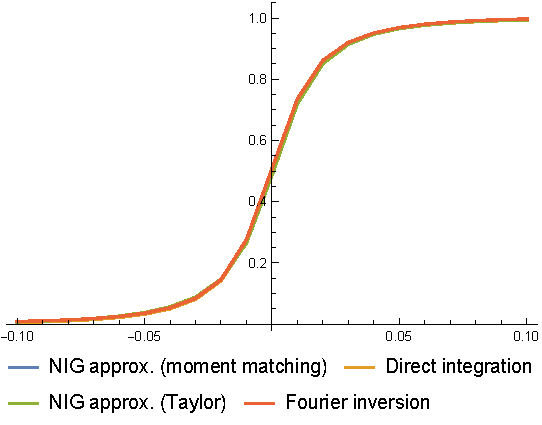
\includegraphics[scale=.8]{_pics/NIG1.pdf}
  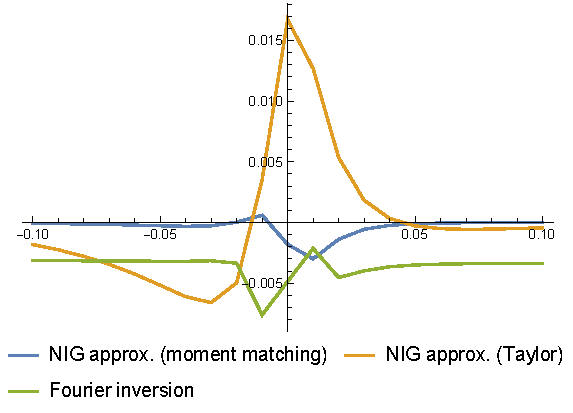
\includegraphics[scale=.8]{_pics/NIG2.pdf}
  \caption{Left: CDF of $R^{0.95}$ using Bitcoin data. Right:
    Difference of different methods to direct integration. CPU times:
    NIG approximation (moment matching): 0.2 seconds plus 18.6 seconds
    for parameter calibration; Direct integration: 82 seconds; NIG 
    approximation (Taylor): 0.18 seconds; Fourier inversion: 0.034
    seconds plus 1.55 seconds to generate smooth density function.}
  \label{fig:NIGs}
\end{figure}

Figure \ref{fig:NIGs} shows an example of the distribution of
$R^{0.95}$ for the different approximations as well as their error
relative to direct integration. It turns out that the NIG
moment-matching approximation performs best in terms of the error,
while the Taylor approximation performs worst. Taking into account CPU
times, the Fourier inversion technique performs best in terms of
balancing error and CPU time. 



\clearpage%
\natp{\em [The definition below is one way of introducing the
  elliptical copula, but not the most practical one for our
  purposes.]}

\begin{definition}
  Elliptical Distribution.  The $d$-dimensional random vector
  $\pmb{y}$ has an elliptical distribution if and only if the
  characteristic function
  $\pmb{t} \mapsto \mathbb{E}\{\exp(i\pmb{t}^\top \pmb{y})\}$ with
  $\pmb{t} \in \mathbb{R}^d$ has the representation
  \begin{align}
    \phi_g(\pmb{t}; \pmb{\mu}, \pmb{\Sigma}, \pmb{\nu}) = \exp(i\pmb{t}^\top\pmb{\mu})g(\pmb{t}^\top\pmb{\Sigma}\pmb{t};\pmb{\nu})
  \end{align}
  where $g(\cdot;\nu):[0, \infty[ \mapsto \mathbb{R}$,
  $\nu \in \mathbb{R}^d$, and $\Sigma$ is a symmetric positive
  semidefinite $d\times d$-matrix.
\end{definition}

If $r$ has a density, then the density of $\pmb{y}$ is of the form
\begin{align}
  |\Sigma|^{\frac{1}{2}} g\{(\pmb{y} - \pmb{\mu})^\top \Sigma^{-1}(\pmb{y} - \pmb{\mu})\}.
\end{align}

The function $g(\cdot; \nu)$ is known as characteristic generator,
whereas $\pmb{\nu}$ is parameter that determines the shape, in
particular the tai index of the distribution.





\begin{corollary} \citep[equation 2.12]{fang2018symmetric} If
  $\pmb{y}$ follows an elliptical distribution, then $\pmb{y}$ has a
  stochastic representation
  \begin{align}\label{eq:stochastic-representation}
    \pmb{y} = \pmb{\mu} + r\pmb{A}^\top \pmb{u},
  \end{align}
  where $r \in \mathbb{R}_+$ is independent of $\pmb{u}$
  % \footnote{$\pmb{u}$ is uniformly distributed on
  % $S_d = \{\pmb{u} \in \mathbb{R}^d s.t. ||\pmb{u}|| = 1\}$},
  , and $\pmb{A}^\top\pmb{A}=\pmb{\Sigma}$.
\end{corollary}

\begin{table}[ht]
  \center
  \begin{tabular}{lll}
    Distribution & $r \sim$ & $g(\pmb{t})$\\ \hline
    Gaussian & $\chi_n$ &
  \end{tabular}
  \caption{Generators of Elliptical Distributions summarised
    from~\cite[Chapter 2]{fang2018symmetric}}
  \label{tab:table}
\end{table}


\subsection{t-copulae}\label{subsec:t-copulae}
The t copula is to represent the dependency structure by t distribution~\citep{fang2002meta, embrechts2002correlation}.
\cite{demarta2005t} extend this idea to skewed t copula and grouped t copula to allow more flexibility in the modelling of dependency structure.

\subsubsection{Vanilla t-copula}\label{subsec:vanilla-t-copula}
The t-copula is
\begin{align}
    C^t_{\nu, \Sigma}(x) =
    \int_{-\infty}^{t_\nu^{-1}(x_1)} \dots \int_{-\infty}^{t_\nu^{-1}(x_n)}
    \frac{\Gamma\left\{ \frac{\nu + i}{2}\right\}}{\Gamma \left\{\frac{\nu}{2}\right\} (\pi \nu)^{i/2}|\Sigma|^{1/2}}
    \left(
    1+ \frac{y^\top \Sigma^{-1}y}{\nu}
    \right)^{-\frac{\nu + i}{2}}
    dy_1 \dots dy_n,
    \end{align}
where $t^{-1}_\nu$ is the quantile function of a univariate student-t distribution with degree of freedom $\nu$.

\subsubsection{Skewed t copula}\label{subsec:skewed-t-copula}
Mean variance mixture

\subsubsection{Double-t copula}\label{subsec:double-t-copula}
\natp{\em [It is OK to introduce the copula without any reference to CDO's.]}
\cite{hull2006valuing} present an alternative way to the Gaussian copula for valuing CDO tranches.
The double-t copula model is a weighted sum of a common (or market)
variable $M$ and a idiosyncratic variable $Z_i$. \natp{\em [They are
  $t$-distributed, right?]}
The double-t copula is
\begin{align} \label{eq:one-fator-model}
X_i = w_i M + \sqrt{1-w_i^2} Z_i
\end{align}
where $M$ and $Z_i$ are independent random variables with zero mean and unit variance, and $X_i$ is an indicator variable for $i^\text{th}$ asset.
The authors map the time to default of the $i^\text{th}$ obligor, $t_i$, to $X_i$,
\begin{align}
    F_{X_i}(x) = F_{t_i}(t).
    \end{align}
In our case, we map $X_i$ to log-returns of portfolio constituents,
\begin{align}
    F_{X_1}(x) = F_{r^S}(s) \text{ and } F_{X_2}(x) = F_{r^F}(t).
    \end{align}
This is also known as percentile-to-percentile
mapping\citep{hull2006defining}.

\natp{\em [The percentile-to-percentile mapping is just the property
  that applying the cdf to a random variable yields a $U(0,1)$
  variable:
  \begin{equation*}
    F(x) = \p(X\leq x) = \p(F(X) \leq F(x)) = \p(U\leq F(x)),
  \end{equation*}
  since by definition, $U\sim U(0,1)$ fulfills $\p(U\leq u)=u$, $0\leq
  u\leq 1$. This could be introduced when copulas and Sklar's Theorem
  are introduced. 
]}
The reason for this mapping is to turn incomprehensible dependency structures into known structure.

\subsubsection{Normal Inverse Gaussian Copula}
Normal Inverse Gaussian (NIG) distribution is a flexible 4-parameter distribution that can produce fat tails and skewness, unlike student-t distribution,
NIG's convolution is stable under certain conditions and the CDF, PDF and quantile function can still be computed sufficiently fast~\cite[chapter 5]{schlosser2011pricing}.
NIG distribution is a mixture of normal and inverse Gaussian distribution.
\begin{definition} Inverse Gaussian Distribution.
    A non-negative random variable $Y$ has an Inverse Gaussian (IG) distribution with parameters $\alpha >0$ and $\beta >0$ if its density funcion is of the form
    \begin{align}
        f_\text{IG}(y; \alpha, \beta) = \frac{\alpha}{\sqrt{2\pi \beta}}y^{-1.5} \exp\left\{
        -\frac{(\alpha - \beta z)^2}{2\beta z}
        \right\}
    \end{align}
    The corresponding distribution function is:
        \begin{align}
        F_\text{IG}(y; \alpha, \beta) = \frac{\alpha}{\sqrt{2\pi \beta}}
        \int_0^y z^{-1.5} \exp\left\{
        -\frac{(\alpha - \beta z)^2}{2\beta z}
        \right\}
            dz.
    \end{align}
    We write $Y \sim \text{IG}(\alpha, \beta)$.
    \end{definition}

\begin{definition} Normal Inverse Gaussian Distribution.
    A random variable $X$ has an Normal Inverse Gaussian (NIG) distribution with parameters $\alpha$, $\beta$, $\mu$ and $\delta$ if its density funcion is of the form
    \begin{align}
        X|Y=y &\sim \Phi(\mu + \beta y, y)\\
            Y &\sim \text{IG}(\delta \gamma, \gamma^2) \text{ with } \gamma \overset{\text{def}}{=}\sqrt{\alpha^2-\beta^2}
    \end{align}
    The corresponding distribution function is:
        \begin{align}
        F_\text{NIG}(y; \alpha, \beta) = \frac{\alpha}{\sqrt{2\pi \beta}}
        \int_0^y z^{-1.5} \exp\left\{
        -\frac{(\alpha - \beta z)^2}{2\beta z}
        \right\}
            dz.
    \end{align}
    \end{definition}


%%% Local Variables: 
%%% mode: latex
%%% TeX-master: "notes.tex"
%%% End: 




%\subsection{Extreme-value copulae}\label{subsec:extreme-value-copulae}


\newpage
\section{Estimation}
%! Author = francis
%! Date = 30.10.20


\subsection{Simulated Method of Moments}\label{subsec:simulated-method-of-moments}
This method is suggested by Oh and Patton (2013).
In this setting, rank correlation e.g. Spearman's $\rho$ or Kendall's $\tau$,
and quantile dependence measures at different levels $\lambda_q$
are calibrated against their empirical counterparts.\medskip

Spearman's rho, Kendall's tau, and quantile dependence of a pair $(X,Y)$
with copula $C$ are defined as
\begin{align}
  \rho_S &= 12 \int\int_{I^2} C_{\bm{\theta}}(u,v)\, \dd u\, \dd v-3\label{eq:rho_S}\\
  \tau_K &= 4\mathbb{E}[C_{\bm{\theta}}\{F_X(x), F_Y(y)\}]-1,\\
  \lambda_q &=
  \begin{cases}
    \p(F_X(X)\leq q| F_Y(Y)\leq q) = \displaystyle \frac{C_{\bm{\theta}}(q,q)}{q},
    &\text{ if } q\in (0,0.5],\\
    \p(F_X(X)>q|F_Y(Y)>q) =\displaystyle \frac{1-2q+C_{\bm{\theta}}(q,q)} {1-q},
    &\text{ if } q\in (0.5,1).
  \end{cases}
\end{align}\medskip
The empirical counterparts are
\begin{align*}
  \hat\rho_S &= \frac{12}{n} \sum_{k=1}^n \hat F_X(x_k) \hat F_Y(y_k)
               -3,\\
  \hat\tau_K &= \frac{4}{n}\sum_{k=1}^n \hat{C}\{\hat{F}_X(x_i),\hat{F}_X(y_i)\} -1 ,\\
  \hat\lambda_q &=
                  \begin{cases}
                    \displaystyle\frac{1}{n} \sum_{k=1}^n \frac{\1_{\{\hat
                        F_X(x_k)\leq q, \hat F_Y(y_k)\leq q\}}} {q},
                    &\text { if } q\in (0, 0.5],\\
                    \displaystyle \frac{1}{n} \sum_{k=1}^n
                    \frac{\1_{\{\hat F_X(x_k)>q, \hat F_Y(y_k)>q\}}}
                    {1-q}, &\text { if } q\in (0.5,1).
                  \end{cases},
\end{align*}
where $\hat{F}(x) := \frac{1}{n}\sum_{k=1}^n 1_{\{x_i\leq x\}}$ and
$\hat{C}(u,v) := \frac{1}{n}\sum_{k=1}^n 1_{\{u_i\leq u, v_i\leq v\}}$.\medskip

We denote $\tilde{\bm{m}}(\bm{\theta})$ be a $m$-dimensional vector of dependence measures according the the
dependence parameters $\bm{\theta}$,and  $\hat{\bm{m}}$ be the corresponding empirical counterpart.
The difference between dependence measures and their counterpart is denoted by
\begin{align*}
    \bm{g}(\bm{\theta}) = \hat{\bm{m}} - \tilde{\bm{m}}(\bm{\theta}).
\end{align*}\medskip

The SMM estimator is
\begin{align*}
    \hat{\bm{\theta}} = \argmin_{\bm{\theta}\in \bm{\Theta}} \bm{g}(\bm{\theta})^\intercal
    \hat{\bm{W}}
     \bm{g}(\bm{\theta}),
\end{align*}
where $\hat{W}$ is some positive definite weigh matrix.\medskip

In this work, we use $\tilde{\bm{m}}(\bm{\theta}) = (\rho_S, \lambda_{0.05}, \lambda_{0.1},
\lambda_{0.9}, \lambda_{0.95})^\intercal$
for calibration of Bitcoin price and CME Bitcoin future.

\subsection{Maximum Likelihood Estimation}\label{subsec:maximum-likelihood-estimation}
By Sklar's theorem, the joint density of a $d$-dimensional random variable $\bm{X}$ with sample size $n$ can be written as
\begin{align}
    \bm{f}_{\bm{X}}(x_1, ..., x_d) = \bm{c}\{F_{X_1}(x_1), ..., F_{X_d}(x_d)\} \prod_{j=1}^d f_{X_i}(x_i).
    \end{align}
We follow the treatment of MLE documented in section 10.1 of \citet{joe1997multivariate}, namely the inference functions for margins or IFM method.
The log-likelihood $\sum^n_{i=1}f_{\bm{X}}(X_{i,1}, ..., X_{i,d})$ can be decomposed into dependence part and marginal part,
\begin{align}
    L(\bm{\theta}) &= \sum_{i=1}^n \bm{c}\{F_{X_1}(x_{i,1};\bm{\delta}_1), ..., F_{X_d}(x_{i,d}; \bm{\delta}_d);\bm{\gamma}\}
    + \sum_{i=1}^n \sum_{j=1}^d f_{X_j}(x_{i,j};\bm{\delta}_j)
    &= L_C(\bm{\delta}_1, ..., \bm{\delta}_d, \bm{\gamma}) + \sum_{j=1}^d L_j(\bm{\delta}_j)
    \end{align}
where $\bm{\delta}_j$ is the parameter of the $j$-th margin, $\bm{\gamma}$ is the parameter of the parametric copula, and
$\bm{\theta} = (\bm{\delta}_1,..., \bm{\delta}_d, \bm{\gamma})$.

Instead of searching the $\bm{\theta}$ is a high dimensional space, \citet{joe1997multivariate} suggests to
search for $\hat{\bm{\delta}_1},..., \hat{\bm{\delta}_d}$ that maximize $L_1(\bm{\delta}_1), ..., L_d(\bm{\delta}_d)$,
then search for $\hat{\bm{\gamma}}$ that maximize $L_C(\hat{\bm{\delta}_1},..., \hat{\bm{\delta}_d}, \bm{\gamma})$.

That is, under regularity conditions, $(\hat{\bm{\delta}_1},..., \hat{\bm{\delta}_d}, \hat{\bm{\gamma}})$ is the solution of
\begin{align}
    \left( \frac{\partial L_1}{\partial \bm{\delta}_1}, ..., \frac{\partial L_d}{\partial \bm{\delta}_d},
    \frac{\partial L_C}{\partial \bm{\gamma}}\right) = \bm{0}.
    \end{align}

However, the IFM requires making assumption to the distribution of of the margins.
\citet{genest1995semiparametric} suggests to replace the estimation of marginals parameters estimation by non-parameteric estimation.
Given non-parametric estimator $\hat{F}_i$ of the margins $F_i$, the estimator of the dependence parameters $\bm{\gamma}$ is
\begin{align}
    \hat{\bm{\gamma}} = \argmax_{\bm{\gamma}} \sum_{i=1}^n \bm{c}\{ \hat{F}_{X_1}(x_{i,1}), ..., \hat{F}_{X_d}(x_{i,d});\bm{\gamma}\}.
    \end{align}



%With the decomposition, the MLE estimator for a bivariate parametric copula is
%\begin{align}
%    \hat{\bm{\theta}} = \argmax_{\bm{\theta} \in \bm{\Theta}} l(X_1,X_2; \bm{\theta}), \label{eq:EMLE}
%    \end{align}
%where
%\begin{align}
%    l(X_1,X_2; \bm{\theta}) = \sum_{i=1}^n \log c(x_{i,1}, x_{i,2};\bm{\theta}). \label{eq:Likelihood}
%    \end{align}\medskip

%Procedure of maximising equation~\ref{eq:EMLE} as a whole is called exact maximum likelihood method.
%Leveraging the attractive feature of copula that one can model the dependence structure and marginals separately,
%we rewrite~\ref{eq:Likelihood} into canonical expression
%\begin{align}
%    l(X,Y; \bm{\theta}) = \sum_{k=1}^n \log c\{F_X(x_i; \delta_X), F_Y(y_i; \delta_Y); \bm{\gamma}\}
%    + \sum_{k=1}^n \log f_X(x_i; \bm{\delta}_X) + \sum_{k=1}^n \log f_X(y_i; \bm{\delta}_Y),
%    \end{align}
%where the $\bm{\gamma}$ is the dependence parameter in the copula and $\bm{\delta}$ is the parameters in the margins.\medskip
%
%The inference-functions for margins (IFM) approach by Joe is a two step procedure of maximising~\ref{eq:EMLE}.
%The approach calibrate first the $\bm{\delta}$s and then the  $\bm{\gamma}$.\medskip
%
%Similar to the IFM approach, pseudo-maximum likelihood approach by Genest and Rivest (1993) replace the parametric margins by
%empirical estimates, we rewrite \ref{eq:Likelihood} again with
%\begin{align}
%    l(X,Y; \bm{\theta}) = \sum_{k=1}^n \log c(u_i, v_i;\bm{\gamma}),
%    \end{align}
%where $u_i = \hat{F}_X(x_i)$ and $v_i = \hat{F}_Y(y_i)$.

\subsection{Comparison}
Both the simulated method of moments and the maximum likelihood estimation are unbiased and
proven to give good fits.
The problem remain is which procedure is more suitable for hedging.
%Cryptocurrencies are known to be very volatile.
Sample and fitted quantile dependence for Bitcoin and CME future.

%\begin{figure}[th]
%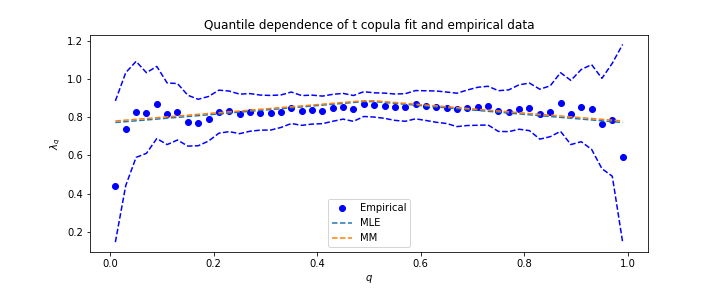
\includegraphics[width=\textwidth]{_pics/t Copula quantile dependence.png}
%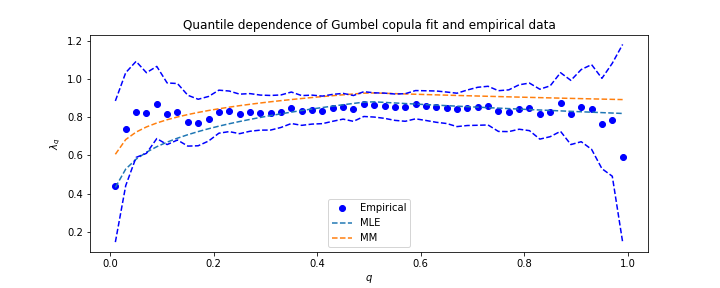
\includegraphics[width=\textwidth]{_pics/Gumbel Copula quantile dependence.png}
%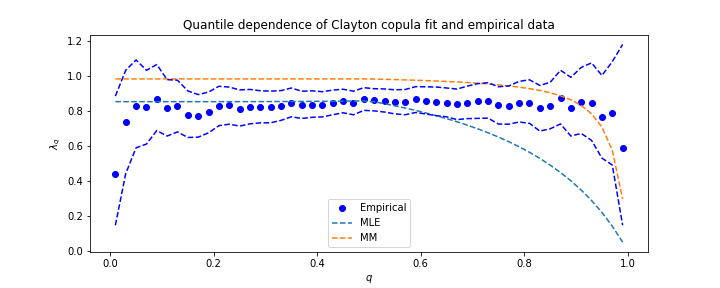
\includegraphics[width=\textwidth]{_pics/Clayton Copula quantile dependence.png}
%  \caption{}
%\label{fig:quantile dependence1}
%\end{figure}


The MM estimation perform just as we decided: match the upper and lower quantile dependence.




%
%
%\subsection{Two-Stage Estimation}\label{subsec:two-stage-estimation}
%~\cite{joe2005asymptotic} study the efficiency of a two-stage estimation procedure of copula estimation.
%The authors also call this method inference function for margins IFM.
%
%\textbf{Pros}
%\begin{enumerate}
%    \item Almost as efficient as MLE methods but easier to be implemented
%    \item Yields an asymptotically Gaussian, unbiased estimate
%\end{enumerate}
%
%\textbf{Cons}
%\begin{enumerate}
%    \item Subject to specification of marginals \cite{kim2007comparison}
%\end{enumerate}
%
%Our data
%\begin{align}
%    \pmb{y} = \begin{bmatrix}
%                  y_{11} & \cdots & y_{1i}\\
%                  \vdots & \ddots & \vdots \\
%                  y_{n1} & \cdots & y_{ni}
%                  \end{bmatrix}
%    \end{align}
%Let $F$ and $f$ be the joint cdf and joint density of $\pmb{y}$ with parameters $\pmb{\delta}$,
%and let $F_i$ and $f_i$ be the marginal cdf and marginal density for the $i^\text{th}$ random variable with parameters $\pmb{\theta}_i$, we have
%\begin{align}
%    f(\pmb{y}; \pmb{\theta}_1, \pmb{\theta}_2,\dots \pmb{\theta}_i, \pmb{\delta}) =
%    c\{F_1(\pmb{y}_1;\pmb{\theta}_1), F_2(\pmb{y}_2; \pmb{\theta}_2), \dots, F_i(\pmb{y}_1;\pmb{\theta}_i); \pmb{\delta}\}
%    \prod^i_{j=1}f_i(\pmb{y}_j;\pmb{\theta}_j)
%    \end{align}
%
%For a sample of size $n$, the log-likelihood of functions of the $i^\text{th}$ univariate margin is
%\begin{align}
%    L_i(\theta_i) = \sum^n_{m=1} \log f_i(y_{mi}; \theta_i),
%    \end{align}
%
%and the log-likelihood function for the joint distribution is
%\begin{align}
%    L(\delta, \theta_1, \theta_2, \dots, \theta_i) = \sum^n_{m=1}\sum^i_{j=1} \log f(y_{mj}; \delta, \theta_1, \theta_2, ..., \theta_i)
%    \end{align}
%
%In most cases, one does not have closed form estimators and numerical techniques are needed.
%Numerical ML estimation difficulty increase when the total number of parameters increases.
%The two-stage estimation is designed to overcome this problem.
%
%The two-stage procedure is
%\begin{enumerate}
%    \item estimate the univariate parameters from separate univariate likelihoods to get $\tilde{\pmb{\theta}_1}, ..., \tilde{\pmb{\theta}_i}$
%    \item maximize $L(\pmb{\delta}, \tilde{\pmb{\theta}_1}, \dots, \tilde{\pmb{\theta}_i})$ over $\pmb{\delta}$ to get $\tilde{\pmb{\delta}}$
%    \end{enumerate}
%
%Under regularity conditions
%\footnote{Regularity conditions include
%1. $\exists \frac{\partial \log f(x;\theta)}{\partial \theta}, \frac{\partial^2 \log f(x;\theta)}{\partial \theta^2}, \frac{\partial^3 \log f(x;\theta)}{\partial \theta^3}$ for all $x$;
%2. $\exists g(x), h(x) and H(x)$ such that for $\theta$ in a neighborhood $N(\theta_0)$ the relations
%$\left|\frac{\partial f(x;\theta)}{\partial theta}\right| \leq g(x)$,
%$\left|\frac{\partial^2 f(x;\theta)}{\partial \theta^2}\right| \leq h(x)$,
%$\left|\frac{\partial^3 f(x;\theta)}{\partial \theta^3}\right| \leq H(x)$ hold for all $x$, and
%$\int g(x) dx < \infty$, $\int h(x) dx < \infty$, $\mathbb{E}_\theta \{H(X)\} < \infty$ for $\theta \in N(\theta_0)$;
%3. For each $\theta \in \Theta$, $0< \mathbb{E}_\theta \left\{
%\left(
%\frac{\partial \log f(X;\theta)}{\partial \theta}
%\right)^2
%\right\}$. For detail see section 4.2.2 of~\cite{serfling2009approximation}}
%, $(\pmb{\tilde{\theta}}_1,\dots \pmb{\tilde{\theta}}_i, \pmb{\tilde{\delta}})$ is the solution of
%\begin{align}
%    (\partial L_1 / \partial \pmb{\theta}^\intercal_1,
%    \dots, \partial L_i / \partial \pmb{\theta}^\intercal_i, \partial L / \partial \pmb{\pmb{\delta}}^\intercal_1) = \pmb{0}
%    \end{align}
%
%For comparison, if we optimize $L$ directly without the two-stage procedure (i.e.~MLE), we solve for
%\begin{align}
%    (\partial L / \partial \pmb{\theta}^\intercal_1,
%    \dots, \partial L / \partial \pmb{\theta}^\intercal_i, \partial L / \partial \pmb{\pmb{\delta}}^\intercal_1) = \pmb{0}
%    \end{align}
%
%We denote the two solutions as
%$\tilde{\pmb{\eta}} = (\pmb{\tilde{\theta}}_1,\dots \pmb{\tilde{\theta}}_i, \pmb{\tilde{\delta}})$ for two-stage procedure;
%$\hat{\pmb{\eta}} =(\pmb{\hat{\theta}}_1,\dots \pmb{\hat{\theta}}_i, \pmb{\hat{\delta}})$ for MLE procedure.
%and compare the asymptotic relative efficiency of $\tilde{\pmb{\eta}}$ and $\hat{\pmb{\eta}}$.
%
%Asymptotics: yet to be done.\\
%~\cite{kim2007comparison} show the estimation of $\pmb{\theta}$ may be seriously affected.
%They compare the two-stage approach and Canonical Maximum Likelihood Method by simulation and
%conclude that Canonical Maximum Likelihood is prefered from a computational statistics and data analysis point of view.
%
%\subsection{Canonical Maximum Likelihood Method}\label{subsec:canonical-maximum-likelihood-method}
%This approach was studied by~\cite{genest1995semiparametric} and~\cite{shih1995inferences}.
%One estimates the margins using empirical CDF
%\begin{align}F_X(x)=\frac{1}{n+1}\sum_{i=1}^n 1(X_i \leq x)\end{align},
%
%we maximize the log-likelihood
%\begin{align}
%    L(\delta) = \sum_{i=1}^n \log [c_\delta \{F_X(X_i), F_Y(Y_i)\}]
%    \end{align}
%
%This procedure does not require specification of marginals.
%
%
%
%
%
%%also by Wang and Ding, 2000; Tsukahara, 2005
%%This is also known as pseudo maximum likelihood (PML) and as canonical maximum likelihood (see Cherubini et al., 2004)
%%
%%Genest and Werker (2002) obtained conditions under which the PMLE is asymptotically efficient.
%%
%%



\newpage
\bibliographystyle{abbrvnamed} %
\bibliography{finance} %
\end{document}

%%% Local Variables: 
%%% mode: latex
%%% TeX-master: t
%%% End: 
